\section{Elektroplanung und Realisierung \textcolor{gray}{(Nikolaj Voglauer)}}

\subsection{Elektroplanung}
\label{sec:Elektroplanung}

\subsubsection{Einleitung - Grundanforderungen}
    Die Zielsetzung bei der elektrischen Planung, war es eine Lösung zu finden, die einerseits die Anforderungen von Erweiterbarkeit und Mobilität erfüllt und andererseits in der Schule beziehungsweise in der Werkstätte produzierbar ist. Die Elektrik des AFSS befindet sich in einem umgebauten Serverschrank, dessen physische Limitierungen bei der Planung ebenfalls berücksichtigt wurden.\\
    In der Anlage sollten während dem Normalbetrieb alle Komponenten vor elektrischen Störungen geschützt sein. Der Fokus liegt hierbei auf dem Schutz von Messleitungen und Steuerleitungen, denn diese liefern präzise Daten, die nicht verzerrt werden sollen.\\ 
    In der Planung wurde stets darauf geachtet, die elektrischen Komponenten so zu verbauen, dass im Falle eines Fehlers sowohl Personen gut geschützt und betroffene Geräte leicht auszuwechseln sind.\\

\subsubsection{Elektrospezififsche Anforderungen}
\label{sec:Elektrik spezififsche Anforderungen}

    \paragraph{Versorgung}\mbox{}\\
    Zur Verfügung steht dem AFSS ein Starkstromanschluss mit 400V Außenleiterspannung. Damit kann nur der Asynchronmotor für das Fließband direkt angesteuert werden.\\
    Alle anderen Elemente brauchen eine andere Spannungsebene. Die insgesamt sieben Schrittmotoren benötigen 24 V mit einem möglichen Dauersummenstrom von über 20A. Die Steuerlogik besteht aus Siemens-SPS, mit Ein- und Ausgangskarten sowie PTO-Karten und einer ET200 mit ASi-Master. Diese Logik benötigt ebenfalls 24 V und sollen getrennt versorgt werden, um von potentiellen Fehlern geschützt zu sein. Der ASi-Kreis benötigt eine eigene ASi-24V-Versorgung.

    \paragraph{Antriebe}\mbox{}\\
    Angesteuert werden müssen folgende Motoren:
    \begin{itemize}
        \item 1 Asynchronmotor (250 W)
        \item 4 stärkere Schrittmotoren (2 Nm)
        \item 3 schwächere Schrittmotoren (40 Ncm)
    \end{itemize}
    Der Asynchromotor braucht keine Drehzahlregelung und wird über eine Wendeschützschaltung angesteuert. Die Schrittmotoren werden über Schrittmotortreiber angesteuert. Diese Treiber werden von PTO-Karten der SPS gesteuert.

    \paragraph{Sicherheit}\mbox{}\\
    Für die Anlage sind folgende Schutzgeräte ausgelegt:
    \begin{itemize}
        \item Fehlerstromschutzschalter (FI);
        \item Leitungsschutzschalter (LS);
        \item Motorschutzschalter;
        \item Gleichstromsicherungen für jeden Schrittmotor.
    \end{itemize} 
    Um die Anlage bei Fehlern, die potentiell von den elektrischen Schutzeinheiten nicht erkannt werden, nach wie vor abschalten zu können, verfügt die Anlage über mehrere Not-Aus-Schalter. Zwei beim Regal selbst, einen im Schaltschrank und einen am Kommisionierplatz. Diese Positionierung soll es Nutzer:innen ermöglichen, aus jeder Position an der Anlage einen Not-Aus-Schalter zu erreichen.

    \paragraph{Bedienelemente}\mbox{}\\
    Physische Bedienelemente sind beim AFSS ein Schlüsselschalter zur Freigabe und ein Drehtrennschalter für eine manuelle Freischaltungsoption.

    \paragraph{Schaltschrank}\mbox{}\\
    Grundsätzlich haben Schaltschränke genormte Anforderungen (IEC 60208 und IEC 61439).\\
    Dazu gehört eine Auslegung von Verdrahtungskanälen, die die Kabel schützen und Umbauten nicht zusätzlich erschweren sollen. Lose verlegte Kabel sollen unter allen Umständen verhindert werden. Das Gehäuse muss geerdet sein und die inneren Komponenten vor Staub und Schmutz schützen. Bei einem potenziellen Lichtbogen soll der Schaltschrank Personen in der Nähe schützen. Zudem muss der Schrank gegen thermische Einflüsse geschützt sein, gegebenenfalls sollte der Schaltschrank, nach Norm, über eine Belüftung verfügen.\\
    Der gewählte Serverschrank, schützt gegen Staub und Schmutz und enthält eine Lüfteranlage, die die Abwärme von mehreren Gleichrichtern gut abführen kann. Zudem sind die Materialien des Schrankes vor Korrosion geschützt (vgl. \cite{Schaltschrank-Anforderungen}).\\
    Bei der Planung muss beachtet werden, dass die Erdung aller leitungsfähigen Elemente eingehalten wird. Außerdem dürfen Umbauten, wie die Montage von Rädern, keiner der angeführten Anforderungen widersprechen.

    \paragraph{Kabelauslegung}\mbox{}\\
    Beim Auslegen von Kabeln gibt es mehrere Punkte, die beachtet werden müssen:
    \begin{itemize}
        \item Spannungsabfall
        \item Nennstrom
        \item Sicherungskonzept
        \item Verlegeart
        \item Elektromagnetische Verträglichkeit (EMV)
    \end{itemize} 
    Während der Spannungsabfall bei den Längen des AFSS vernachlässigt werden kann, muss besonders auf Schleppkettentauglichkeit geachtet werden. Steuer- und Messkabel müssen entsprechend geschirmt werden und abhängig vom Strom muss der passende Querschnitt gewählt werden. Dabei müssen die Querschnitte auch auf die Schutzautomaten im Stromkreis abgestimmt werden.\\

    \paragraph{Module}\mbox{}\\
    Die Paneele/Module, zur Montage der elektrischen Komponenten, müssen ebenfalls eine umfassende Erdung ermöglichen und mechanisch den Belastungen standhalten. Dabei ist das Gewicht die maßgebliche Belastung. Die Verdrahtungskanäle müssen eine übersichtliche Verdrahtung gewährleisten, die Modularität der Paneele soll vorteilhaft ausgenutzt werden und soll das Projekt nicht unnötig verkomplizieren. Kostentechnisch soll dabei ein möglichst günstiges, aber standhaftes Material gewählt werden.

\subsubsection{Mechanische Planung}
    \paragraph{Schaltschrankrahmen}\mbox{}\\
        \begin{figure}[h]
        \centering
        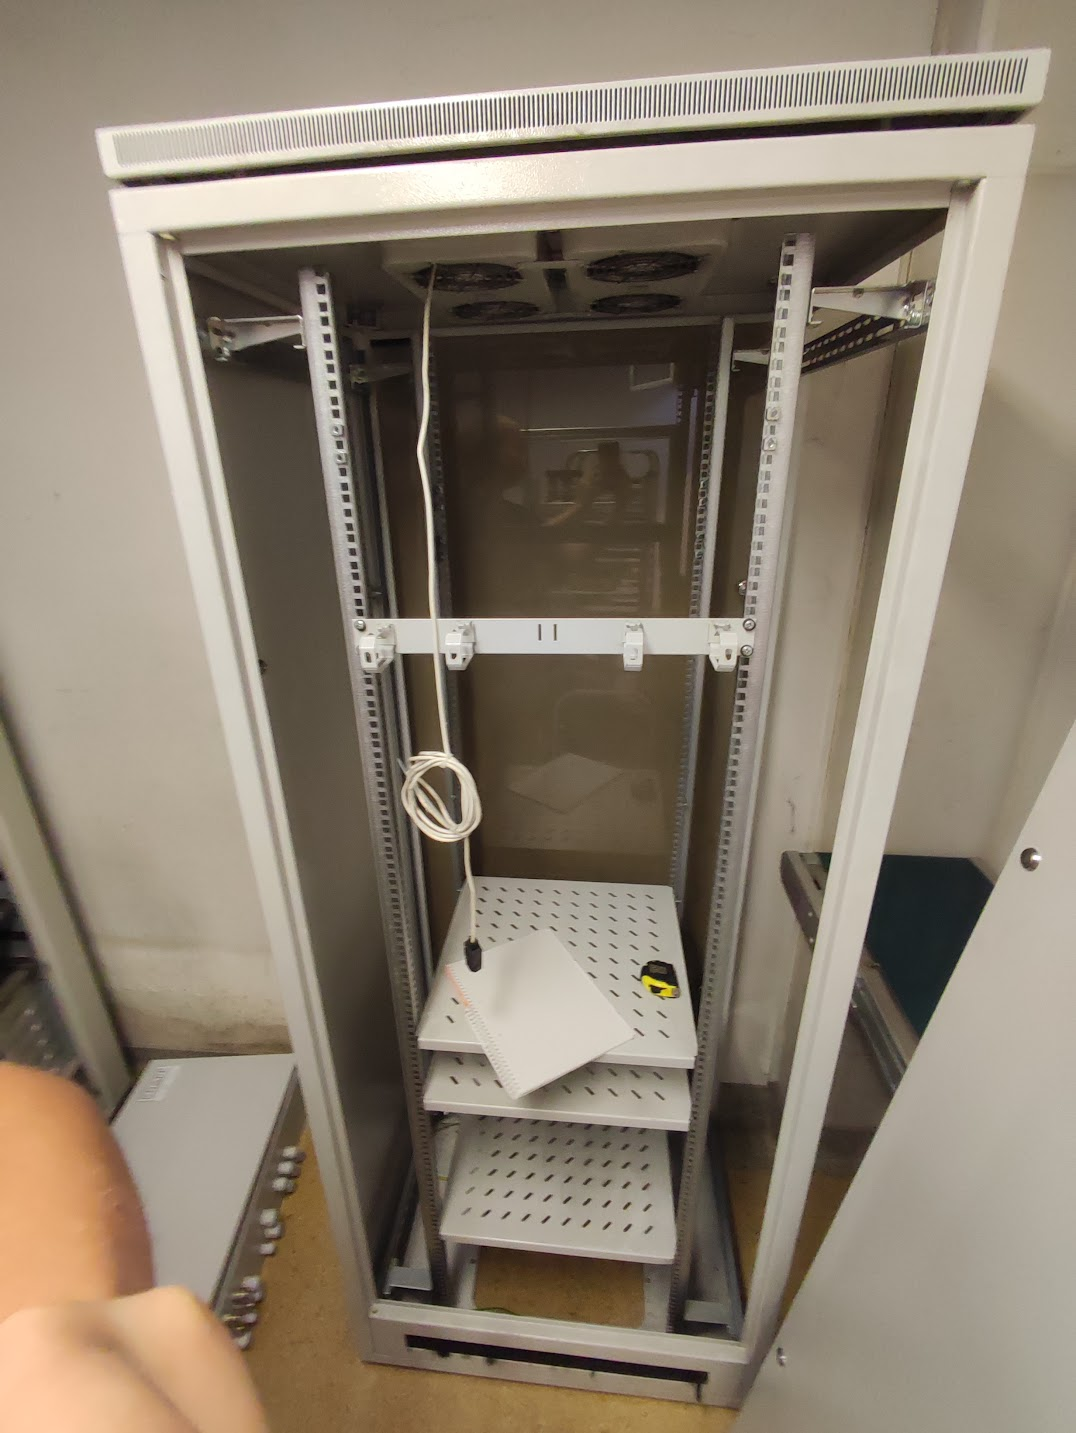
\includegraphics[width=0.5\textwidth]{Vogis Bilder/Serverschrank_original.jpg}
        \caption{Serverschrank bei Übergabe an das AFSS-Team}
        \label{fig:Serverschrank_original}
    \end{figure}
    Bevor man sich den Details des Schaltschrankes widmet, muss zuerst der Rahmen festgelegt werden. Grundsätzlich würde man einen herkömmlichen Schaltschrank verwenden, allerdings sind diese teuer und erfüllen auch nicht die Anforderung der Mobilität. Deswegen wurden mehrere alternative Optionen in Betracht gezogen.\\
    Anfangs wurde der Ansatz verfolgt, die elektrischen Komponenten in den Lagerschrank selbst einzubauen. Dabei hätte man entweder einen eigenen Abteil für die Elektrotechnik einplanen können, der auch mittels entsprechendem Material räumlich getrennt wäre, oder man hätte die Elemente fluide unterbringen können. Damit ist gemeint, dass in dem ganzen Lagerschrank verteilt die elektrischen Komponenten montiert wären.\\
    Die fluide Variante benötigt sorgfältige Planung und auch durchgehende Absprache mit der restlichen mechanischen Planung des AFSS. Dafür hätte man ein kompaktes Design, allerdings wäre das Risiko für Verletzungen und Schäden höher, da die elektrischen Komponenten nur schwer räumlich trennbar wären. Aufbauend auf der fehlenden Sicherheit und der Tatsache, dass die benötigte Kommunikation in einer Entwicklungsphase nicht möglich wäre, wurde diese Option nicht verfolgt.\\
    Wesentlich realistischer ist der Ansatz ein eigenes, kleines Abteil in den Schrank einzubauen. Der Rahmen sowie das Lager wären aus Aluminiumprofilen gebaut und die jeweiligen Seiten mit Kunststoffen verkleidet, um die räumliche Trennung zu gewährleisten. Diese Option ist kommunikationstechnisch möglich, da man sich mit der restlichen mechanischen Planung nur auf die Außenmaße und Position dieses Abteils einigen muss. Allerdings bedeutet ein integriertes Abteil auch weniger Lagerplätze und einen deutlichen Zusatzaufwand in der Realisierung. Diese Variante wurde verworfen, um die Lagerplätze zu maximieren\\
    Auf der weiteren Suche nach einer Alternative zum herkömmlichen Schaltschrank wurde die Möglichkeit, einen alten Serverschrank der Schule (siehe Abbildung \ref{fig:Serverschrank_original}) zu recyceln, erkannt. Ein fertig gebauter Schrank, der im Fehlerfall die Umgebung ausreichend schützt und keine Zusatzkosten mit sich bringt, wurde als beste Option gewählt. Die im Inneren bereits vorhandenen Profilschienen bieten viele Möglichkeiten die Elektrotechnik, zu montieren. Zudem bietet der Innenraum des Serverschrankes viel Platz und auch die Möglichkeit, die Elektrotechnik im Bedarfsfall rasch und einfach zu erweitern, da man die Profilschienen sehr indiviuell nutzen kann.\\
    Es wurde entschieden, den Serverschrank zu einem Schaltschrank umzubauen. Im Zuge des Umbaus wurde der Innenraum umgebaut und der Serverschrank mobil gemacht. 
    \paragraph{Modulprinzip}\mbox{}\\
    Das Innenleben des Schaltschrankes ist in mehrere Module getrennt. Die Anforderungen an diese wurden schon beschrieben, doch ursprünglich waren weitere Alternativen für den Innenraum des Serverschrankes in Diskussion.\\
    Anstatt mehrerer Module, die später genauer beschrieben werden, hätte man eine durchgehende Platte verwenden und diese an den Profilschienen des Serverschrankes festschrauben können. Vorteilhaft an einer durchgängigen Platte wäre gewesen, dass man in der Positionierung der Komponenten mehr Freiheiten gehabt hätte. Die große Platte entfällt als Möglichkeit allerdings insofern, da diese nicht in der Schule produzierbar ist.\\
    Eine andere Option wäre eine plattenlose, bei welcher man die Hutschienen direkt auf die Profilschienen des Serverschrankes montiert. Man spart sich so Platten. Die plattenlose Option ist eine kosteneffiziente Möglichkeit, allerdings gibt es viele Elemente, die im Schaltschrank nicht auf Hutschienen montiert werden können, diese bräuchten immer eine Montageplatte.\\
    Damit ein einheitliches Design eingehalten werden konnte, wurde ein Modulprinzip gewählt. Dieses ermöglicht, alle Elemente, auch für die, die für Hutschienen ungeeignet sind, zu montieren und ist dennoch in der Schule herzustellen.

    \paragraph{Platten-Material}\mbox{}\\
    Für die Materialwahl gab es drei realistische Möglichkeiten: 
    \begin{itemize}
        \item Aluminium;
        \item Dibond;
        \item Kunststoff.
    \end{itemize}
    Die Aluplatten bieten den Vorteil der Leitfähigkeit und somit müsste man nur die Platte erden und die Elemente auf der Platte wären alle dementsprechend geerdet. Bei reinen Kunststoffplatten gibt es keine Leitfähigkeit und zusätzlich bieten die meisten Kunststoffe keine ausreichende mechanische Stabilität.\\
    \begin{figure}[h]
        \centering
        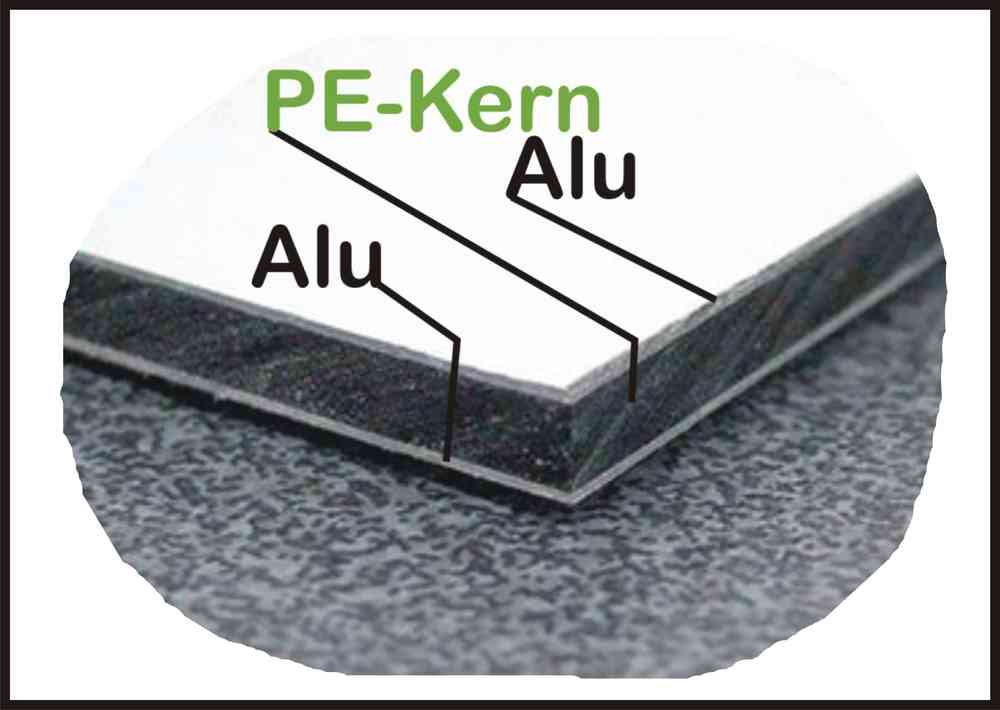
\includegraphics[width=0.5\textwidth]{Dibond_Platten_ml.jpg}
        \caption{Dibond-Platte, Quelle: \cite{Dibond-Platte}}
        \label{fig:Dibond-Platte}
    \end{figure}
    Aluminium erfüllt alle Anforderungen, ist aber teuer und ein wertvoller Werkstoff. Da ein umsichtiger Umgang mit Ressourcen wichtig ist, wurde nach einer Alternative gesucht. Dibond wurde daraufhin als Projektstandard für die Module definiert (siehe Abbildung \ref{fig:Dibond-Platte}). Dieser Stoff besteht aus zwei dünnen Aluminiumplatten, die auf eine Kunststoffplatte aufgepresst werden. Dibond bietet keine elektrische Leitfähigkeit, folglich müssen alle Elemente, wie Hutschienen, zusätzlich geerdet werden. Das leichte Gewicht und die hohe mechanische Stabilität machen Dibond daher zur besten Option.

    \paragraph{Digitaler Zwilling}\mbox{}\\
    Moderner Schaltschrankherstellung begegnen im Herstellungsprozess oft große logistische Probleme. Jeder Prozessschritt ist eine Fehlerquelle und wenn Fehler nicht früh erkannt werden, setzen sich diese fort. Damit zwischen den Prozessschritten keine Kommunikationsprobleme entstehen, setzen viele Hersteller auf das Prinzip des digitalen Zwillings.\\
    Dieser ist im Grunde ein digitaler Schaltschrank, welcher im ersten Prozessschritt, der Planung, ausgeplant wird und im Herstellungsprozess, sei es beim Schrankbau oder bei der Bestückung, aktualisiert und referenziert wird. Das heißt alle Prozessschritte beziehen sich auf denselben Plan bzw. digitalen Zwilling (siehe \ref{fig:digilaerZwilling}).
    \begin{figure}[h]
        \centering
        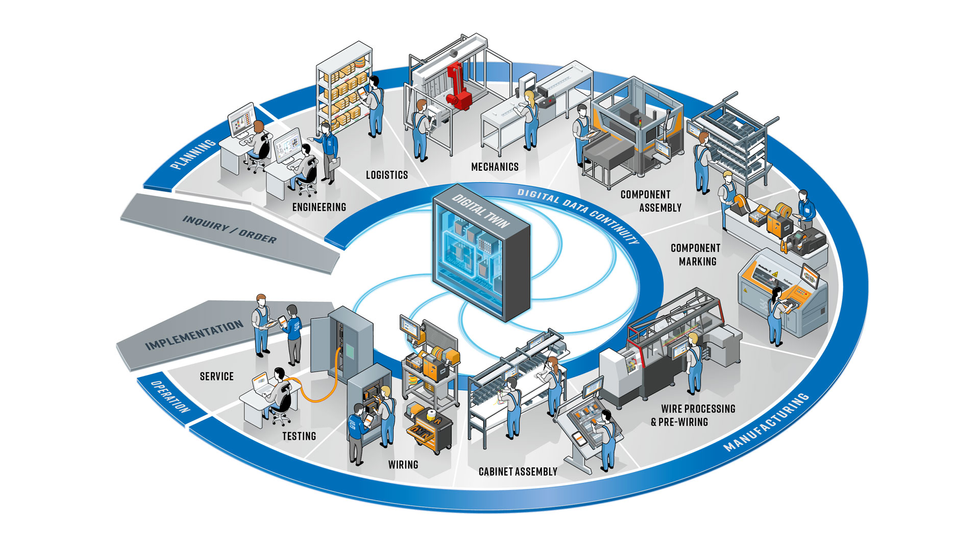
\includegraphics[width=0.9\textwidth]{Cabinet-Building-Komax-SCB-Component-Printer.png}
        \caption{Digitaler Zwilling, Quelle: \cite{digitaler_zwilling_bild}}
        \label{fig:digilaerZwilling}
    \end{figure}
    Es setzt auch ein breites Feld an Firmen auf dieses Prinzip. Firmen wie Weidmüller, Komax, Steinhauer und noch viele mehr haben eine Firmenzusammenarbeit, die ohne einen digitalen Zwilling nicht möglich wäre (vgl. \cite{smart_cabinet_building}). In diesem Fall werden die jeweiligen Prozessschritte meistens von einer neuen Firma übernommen. In diesem Bündnis ist der digitale Zwilling der Schlüssel zum Erfolg. Man kann dieses Prinzip der Dokumentation bzw. Planung als Industriestandard verstehen.\\
    Um den Prozess der Herstellung des Schaltschrankes möglichst nahe an die Praktiken aus der Industrie anzugleichen, wird auch der Schaltschrank des AFSS mithilfe eines digitalen Zwillings geplant. Dieser wird in Fusion360 gezeichnet und soll den Sollzustand des Schaltschrankes abbilden.\\
    Um die Konstruktion zu beginnen, braucht es eine möglichst ausführliche Ausmessung des bereits bestehenden Serverschrankes. Besonders wichtig sind die Elemente, die direkt am Umbau beteiligt sind, wie die Profilschienen (Abstände der Löcher, Abstände der Profilschienen zueinander und detaillierte Abmessungen der Profilschienen selbst), die Türen und die Lüfter.\\

    \paragraph{Digitaler Zwilling - Umsetzung}\mbox{}\\ 

    \begin{figure}[h]
        \centering
        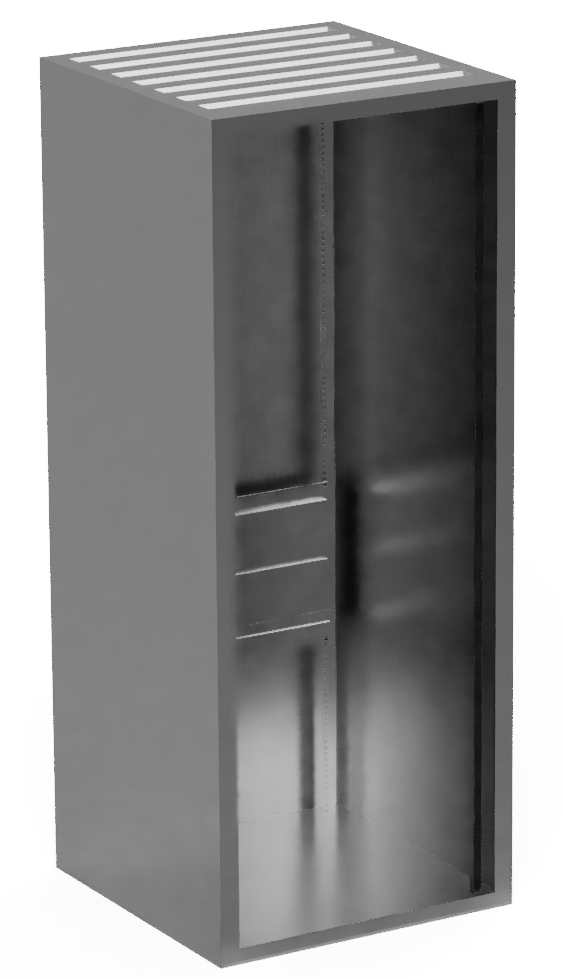
\includegraphics[width=0.3\textwidth]{Prototyp_Serverschrank.PNG}
        \caption{Sommerprototyp eines Serverschrankes}
        \label{fig:Sommerprototyp}
    \end{figure}
    Als Erstes wird der Serverschrank, ausführlich ausgemessen. Äußere Höhe, innere Höhe, äußere Breite, innere Breite und noch viele mehr müssen richtig gemessen werden.    
    Für die Messungen werden Messschieber und bei größeren Abständen Maßbänder verwendet. Um die mechanische Konstruktion zu erleichtern, werden alle Daten digital festgehalten. Während die Messungen des Serverschranks für den finalen digitalen Zwilling wichtig werden, gibt es aber auch noch andere Punkte die berücksichtigt werden müssen. Beispielsweise die Frage, ob das Modulkonzept so möglich sei. Aufgrund dessen und des Umfanges der Diplomarbeit, sowie der begrenzten Zeit, wurde ein erster Entwurf eines Serverschrankes in Fusion360 konstruiert (siehe Abbildung \ref{fig:Sommerprototyp}) und weiters ein Probemodul gezeichnet. Die Maße dieses digitalen Prototyps sind von einem Standard-Serverschrank übernommen.\\
    Dieser Prototyp hat nicht die selben Werte wie der richtige Serverschrank, der dem AFSS zur Verfügung steht. Aufgrund der Prototyp-Konstruktion stand fest, dass das Modulkonzept so umsetzbar war. Weiters wurde festgestellt, wie eine Fusion360 Zeichnung optimaler gestalltet werden kann. Eine Erkenntnis des Prototyps war, dass man den Serverschrank nicht als ein großes Element konstruieren sollte. Wenn ein Fehler spät erkannt wird, ist dieser so gut wie nicht mehr zu beheben. Wenn die Konstruktion allerdings auf viele verschiedene Elemente aufgeteilt wird, dann ist der Schaden bei einem Fehler begrenzt.\\
    Nachdem das Grundprinzip erfolgreich konstruiert wurde, ist der Serverschrank auf Grundlage der echten Maße zu konstruieren gewesen (siehe Abbildung \ref{fig:Clean_Serverschrank}). Die gewonnen Erkenntnisse wurden dabei bestmöglich miteinbezogen.\\    
    \begin{figure}[h]
        \centering
        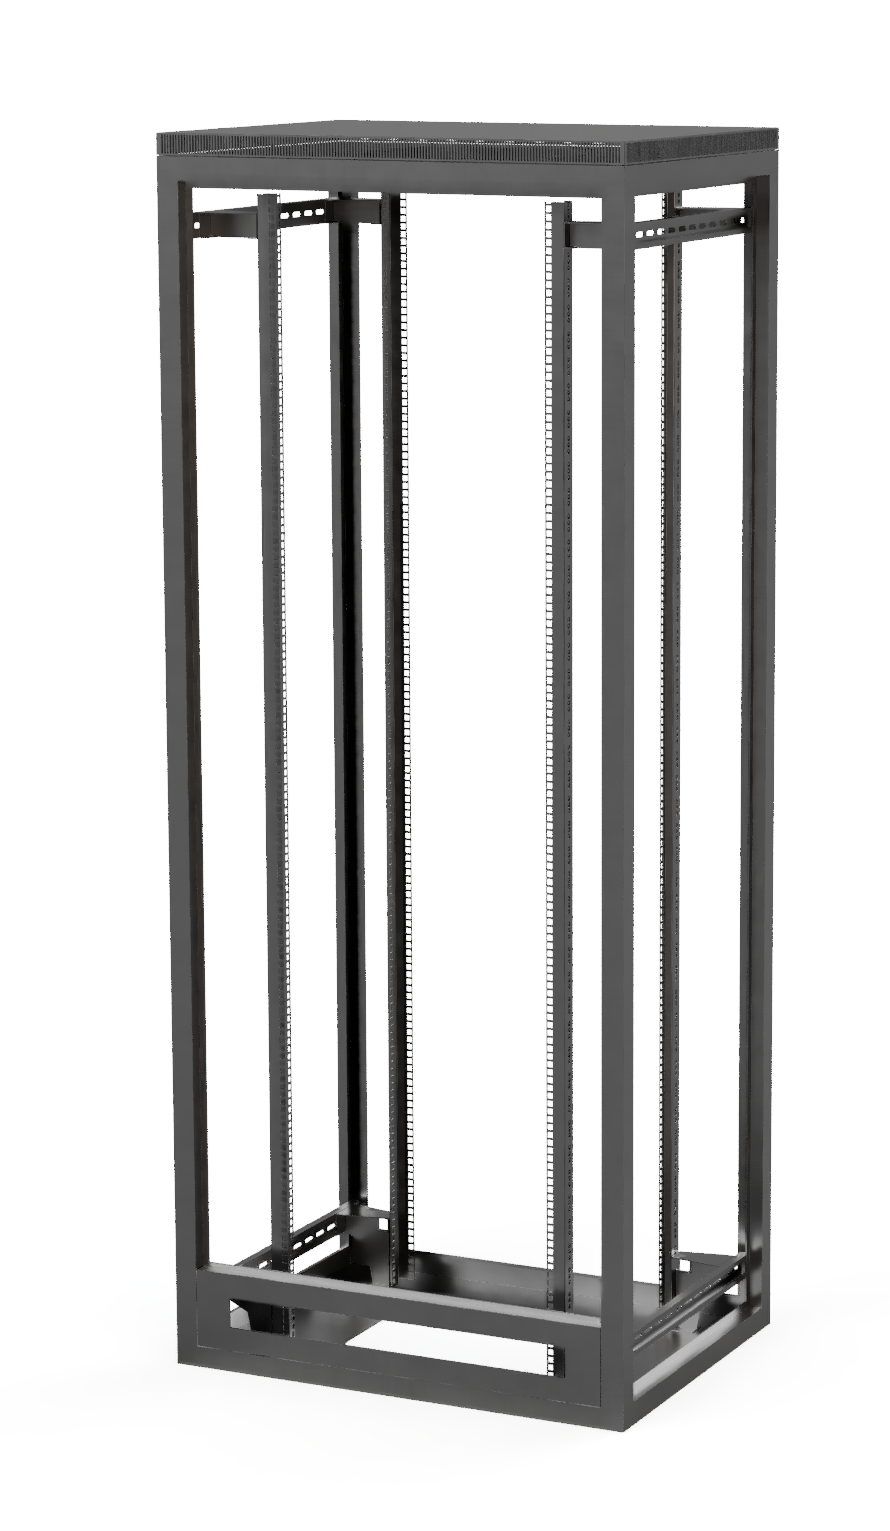
\includegraphics[width=0.35\textwidth]{Schaltschrank_ohne_Module.PNG} 
        \caption{Serverschrank konstruiert}
        \label{fig:Clean_Serverschrank}
    \end{figure}
    Mit dem fertig konstruierten Serverschrank konnte dann die Planung der Module beginnen. Dafür wurde zuerst ein Konzept erstellt, welche elektrischen Baugruppen wo im Schaltschrank platziert werden sollten. Das Konzept richtete sich einerseits nach der Vorgabe, zusammengehörige elektrische Komponenten sollten auf dasselbe Modul kommen und andererseits zusammenhängende Module sollten sich möglichst nahe sein. 
\subsubsection{Grundkonzept der Module}
    \paragraph{Modul 1 - Bedienelemente}\mbox{}\\
    Im Schaltschrank vorhanden sind jeweils ein:
    \begin{itemize}
        \item Not-Aus-Schalter
        \item Schlüsselschalter
        \item Drehtrennschalter
    \end{itemize}
    Diese Elemente sind gemeinsam auf einem Modul verbaut, da sie alle Bedienelemente sind.
    \paragraph{Modul 2 bis 3 - Schutzorgane und Versorgungen}\mbox{}\\
    Direkt unter dem Drehstromschalter liegen die Schutzorgane. Da der Leitungsschutzschalter und der Fehlerstromschutzschalter wenig Platz benötigen, sind auf dem 2. Modul zusätzlich zwei Gleichrichter auf dieselbe Hutschiene gesteckt. Damit besteht das 2. Modul aus Schutzorganen und Gleichrichtern. Auf der Platte ist damit eine durchgängige Hutschine und ein Verdrahtungskanal montiert.\\
    Für die reguläre Versorgung des AFSS werden drei normale Netzteile benötigt. Das Dritte, das Deutronic Netzteil, kann nicht auf eine Hutschine montiert werden und hat zudem einen großen Platzbedarf. Dieses ist auf einem eigenen Modul montiert. In den Leerräumen des 3. Moduls sind Hutschienen mit Reihenklemmen montiert. Diese Reihenklemmen sorgen für eine übersichtliche Verdrahtung der Versogungsleitungen.
    \paragraph{Modul 4 - ASi-Versorgung und DC-Sicherungen}\mbox{}\\
    Konzepttechnisch war das 4. Modul ein Erweiterungsmodul auf welchem Platz gelassen wurde, für potentielle Erweiterungen. Nur eine Ein/Ausgangsbaugruppe von Weidmüller wurde auf eine kleine Hutschiene verplant.\\
    Im Entwicklungsprozess wurde deutlich, dass die PWM-Signalerzeugung, der Ausgangsbaugruppen nicht in der Lage ist ein veränderbares PWM-Signal zu erzeugen. Damit können diese Elemente nicht verwendet werden, zeitgleich wurde erkannt, dass es eine getrennte 24V-Versorgung für den ASi-Kreis geben muss. Deswegen ist im ursprünglichen Erweiterungsbereich dieses Modules ein 24V-ASi-Gleichrichter montiert, der keine Hutschiene benötigt. Anstatt der ursprünglichen Ausgangsbaugruppen sind alle DC-Sicherungen für die Schrittmotoren montiert. Zudem ist auch ein Verdrahtungskanal am Modul.
    \paragraph{Modul 5 - SPS und Sicherungen}\mbox{}\\
    Das 5. Modul beinhaltet die Siemens SPS und die ET 200 SP samt ASi-Master. Für die SPS ist eine Siemens-Profilschiene auf der Platte und für die ET 200 SP eine durchgängige Hutschiene sowie ein anfälliger Verdrahtungskanal. Auf der Hutschiene neben der ET 200 SP sind drei Schrittmotor-Treiber, für die 40 Ncm Schrittmotoren, aufgesteckt.
    \paragraph{Modul 6 - Schrittmotoren}\mbox{}\\
    Für die stärkeren Schrittmotoren werden Treiber verwendet die direkt auf einen Untergund montiert sind. Die vier Treiber sind auf eine eigene Platte gesetzt. Auch auf diesem Modul ist ein Verdrahtungskanal vorhanden.
    \paragraph{Modul 7 - Ausgangsmodul}\mbox{}\\
    Das Ausgangsmodul hat einen Verdrahtungskanal und eine durchgängige Hutschiene. Auf diese Hutschiene sind Elemente wie Motorschütze, Relais und ausreichend Reihenklemmen.
    \paragraph{Modul 8 - Erdungsmodul}\mbox{}\\
    Etwaige Kabel des AFSS haben einen Schirm der geerdet ist. Deswegen ist eine Erdungsplatte nötig die aus leitfähigen Aluminium gemacht ist. Auf dieser ist eine Ankerschiene zur Zugentlastung von Kabeln und Erdung von Leiterschirmen vorhanden. Zudem sind in diesem Modul vier rechteckige Ausfräsungen, für die Buchse vom RJ45-Stecker.
    \begin{figure}[h]
        \centering
        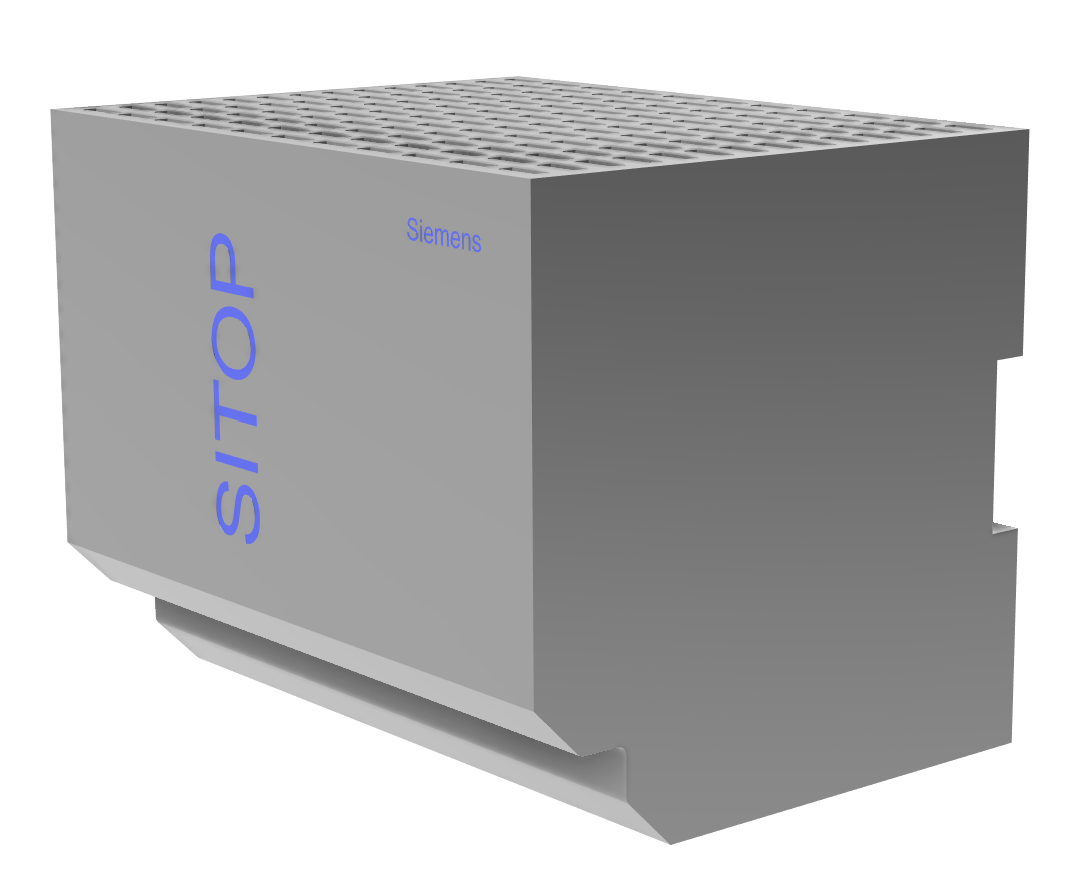
\includegraphics[width=0.3\textwidth]{Vogis Bilder/SITOP_Konstruiert.png}
        \caption{Siemens SITOP in Fusion360}
        \label{fig:SITOP_Konstrueiert}
    \end{figure}
    \paragraph{Module - 3D Konstruktion}\mbox{}\\
    Die einzelnen Module wurden im Anschluss an die Konzeptionierung, in Fusion360 gezeichnet. Dafür wurden zuerst die einzelnen Komponenten wie Hutschienen, Verdrahtungskanäle, Gleichrichter und alle anderen Komponenten als unabhängige Konstruktionen gezeichnet. Mit dieser breiten Bibliothek an Komponenten, konnte man dann einfach und effizient den digitalen Schaltschrank bestücken. Bei den jeweiligen Elementen standen nicht die kleineren Details im Vordergrund, vielmehr wurden die Außenmaße, die Positionen von Montagelöchern oder des Klemmmechanismus für die Hutschiene akkurat abgebildet (siehe Abbildung \ref{fig:SITOP_Konstrueiert}).
    \begin{figure}[h]
        \centering
        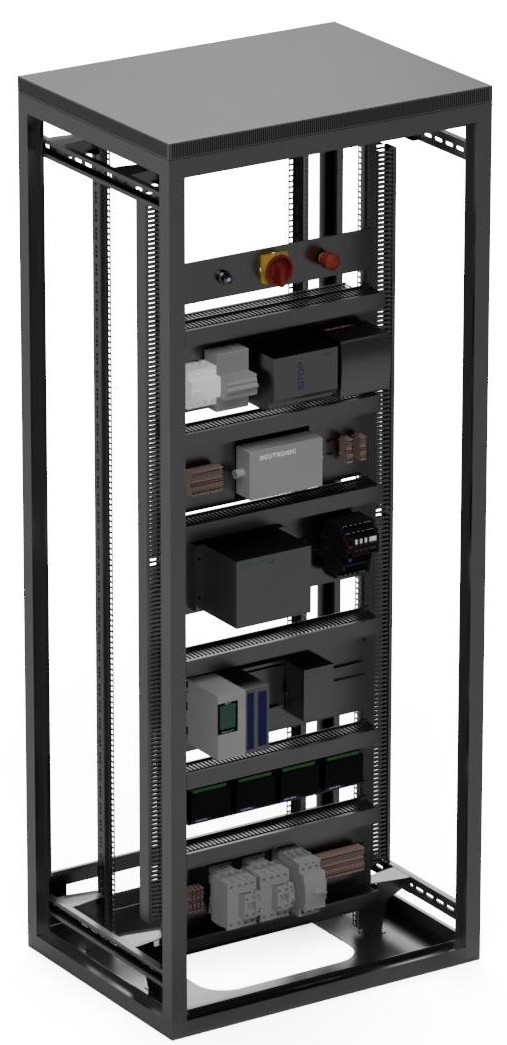
\includegraphics[width=0.4\textwidth]{Vogis Bilder/Bestuekter_Schaltschrank_Fusion.jpg}
        \caption{Der Schaltschrank in Fusion360 gezeichnet}
        \label{fig:Schaltschrank_bestueckt_Fusion}
    \end{figure}
    \paragraph{Fusion360}\mbox{}\\
    Nachdem die einzelnen elektrischen Komponenten gezeichnet waren, wurde in Fusion die erste Platte gezeichnet. Hierbei muss man nicht sofort die richtige Größe abschätzen, da Fusion spätere Änderungen zulässt. Nachdem eine Platte im Serverschrank konstruiert wurde, wurden die Hutschienen und Verdrahtungskanäle eingefügt. Daraufhin wurde die Unterkonstruktion bestückt. Beim Einfügen von Konstruktionen in andere Konstruktionen bleiben die kopierten Elemente mit der originalen Zeichnung verknüpft. Diese Verknüpfung wurde bei den Elementen gelassen, die keine Änderungen erwarten lassen. Bei Komponenten wie einem Verdrahtungskanal sollte man die Verknüpfung trennen um das Element nachträglich zuschneiden zu können. Eine Verknüpfung bedeutet, dass Veränderungen nur in der ursprünglichen Zeichnung getätigt werden können. So wurde jedes Modul der Reihe nach gezeichnet.\\
    Beim Zeichnen und Konstruieren fiel auf, dass die Module aus dem Serverschrank, beziehungsweise Schaltschrank, herausragten. Es wurde festgestellt, dass die Profilschienen nach innen verschoben werden müssen, um zu ermöglichen, dass sich die Wände des Schaltschrankes auch schließen lassen. Die Bauart des Serverschrankes erlaubte eine solche Veränderung.\\ 
    Es wurden, bis auf das Erdungsmodul, alle Module auf diese Art konstruiert. Man konnte schön erkennen, welche Reihenfolgen sinnvoll ist und wie sich welche Komponenten am besten montieren lassen. Beispielsweise wurde ausgetestet, ob bei gewissen elektrischen Komponenten eine vertikale Montage zielführend wäre. In der Abbildung \ref{fig:Schaltschrank_bestueckt_Fusion} sieht man die fertige Konstruktion des Schaltschrankes.\\
    Zu dieser Version des Schaltschrankes ist zu sagen, dass ab der Realisierung des Geplanten, dieser digitale Plan sich fließend transformiert zum digitalen Zwilling. Dieser Zwilling gehört nach der Realisierung konstant gepflegt. Das Erdungsmodul beispielsweise, welches erst mitten in der Realisierung eingeplant und umgesetzt wurde, musste dem digitalen Zwilling nachträglich hinzugefügt werden.
    \paragraph{AutoCAD}\mbox{}\\
    \label{AutoCAD}
    Nachem der digitale Plan/Zwilling vollständig ausgeplant war, mussten die jeweiligen Platten gefräst werden. Um die Platten auch fräsen zu können, mussten diese zuerst als DXF-Datei in Filou-NC eingefügt werden. Dazu mussten die einzelnen Module in AutoCAD nachgezeichnet werden. Idealerweise hätte man hierfür nur die Oberfläche der Platten in Fusion zur Skizze gemacht und diese dann als DXF exportiert. Bei einem nachträglichen Ausmessen der 3D-Konstruktion wurde allerdings festgestellt, dass sich die Plan-Maße der Löcher der Profilschiene nicht mit dem Naturmaß decken. Zudem wurden weitere minimale Abweichungen festgestellt. Keiner der Fehler war so gravierend, dass man die digitale Konstruktion des Schaltschrankes nicht weiterverwenden hätte können, aber für eine präzise Fräsung aufbauend auf der Fusion-Konstruktion waren die Abweichungen zu groß. Deswegen wurden alle Module in AutoCAD sorgfälltig nachgezeichnet.\\     
    Beim Nachzeichnen wurden alle fehlerhaften Maße ausgebessert. Mit den richtigen Maßen wurde festgestellt, dass gewisse Module nicht wie geplant gebaut werden konnten. Beim Modul 6 gingen sich die vier Schrittmotortreiber nicht vertikal nebeneinander aus. Deswegen wurde in AutoCAD einer der Treiber vertikal angeordnet und weiterführend wurde die Änderung auch in Fusion nachgebessert.
    \paragraph{Räder}\mbox{}\\
    In der Transformation vom Serverschrank zum Schaltschrank des AFSS gehört auch, dass der Schrank mobil gemacht wird. Dazu wurden zwei flexible und zwei starre Räder zur Verfügung gestellt. Planungstechnisch wurde diesbezüglich besprochen, dass die Räder direkt an das bestehende Gerüst geschraubt werden. Montiert werden die Räder mit simplen Schrauben und Muttern. Die Räder wurden in AutoCAD nicht gezeichnet, da dies nicht als Zweckerfüllend erachtet wurde.\\
    Nach dargestellter Verplanung ist die Detailzeichnung des Schaltplanes erstellt worden.
    \newpage
\subsubsection{Die elektrischen Komponenten}
\label{sec:Die elektrischen Komponenten}
    Das AFSS verfügt über eine große  Bandbreite elektrischer Komponenten. Jede Art von Elementen ist zur besseren Verständlichkeit kurz aufgelistet (siehe Tabelle \ref{tab:elektrische_komponenten}), bevor im nächsten Kapitel die jeweiligen Funktionen beleuchtet werden.
    \paragraph{Übersicht der Komponenten}\mbox{}
    \begin{table}[h!]
        \centering
        \begin{tabular}{|l|l|l|}
            \hline
            \textbf{Allgemeine Bezeichnung} & \textbf{Typenbezeichnung} & \textbf{Funktion} \\ \hline
            Trennschalter & / & Manuelle Trennung vom Netz \\ \hline
            Schlüsselschalter & / & Freigabeschalter \\ \hline
            Not-Aus-Schalter & / & Manueller Not-Aus \\ \hline
            Motorschutzschalter & / & Schutz für ASM \\ \hline
            FI & TYP A 30mA & Fehlerstromschutzschalter \\ \hline
            LS & C13 & Leitungsschutzschalter \\ \hline
            SITOP & 6EP1436-3BA00-8AA0 & 400/24V Netzteil \\ \hline
            Deutronic & DP500IP/3-24 & 400/24V Netzteil \\ \hline
            Meanwell-Netzteil & DRT-240-24 & 400/24V Netzteil \\ \hline
            Telemecanique & TSX-SUP-A054 & 400/24V ASi-Netzteil \\ \hline
            SPS & 6ES7515-2AN03-0AB0 & Steuereinheit \\ \hline
            SPS-DI-Karte & 6ES7521-1BL00-0AB0 & Digitale Eingänge \\ \hline
            SPS-DO-Karte & 6ES7522-1BL01-0AB0 & Digitale Ausgänge \\ \hline
            SPS-PTO-Karte & 6ES7553-1AA00-0AB0 & Erzeugung von PWM-Signalen \\ \hline
            ET 200 SP& 6ES7155-6AU01-0CN0 & dezentrale Peripherie \\ \hline
            ET 200 Busadapter & 6ES7193-6AR00-0AA0 & Busanschluss \\ \hline
            ET 200 ASi Master & 3RK7137-6SA00-0BC1 & ASi-Master \\ \hline
            ET 200 Steckadbater & 6ES7193-6BP20-0DC0 & Steckadapter für ASi-Master \\ \hline
            ASi-Slaves & 3RK2200-0CE02-0AA2 & Nimmt Sensoren auf \\ \hline
            Feed-In-Modul & 2081870000 & Eingang zu DC-Sicherungen \\ \hline            
            Service-Schnittstelle & IE-FC-SET-SPDEK001-KY-P & Schnittstelle für externen Zugriff \\ \hline
            8A-DC-Sicherung & 2080600000 & Sicherung von SM \\ \hline
            2A-DC-Sicherung & 2080480000 & Sicherung von SM \\ \hline
            SM-Treiber groß & CL57T(V4.0) & Ansteuerung von SM \\ \hline
            SM-Treiber klein & TB6560 & Ansteuerung von SM \\ \hline
            SM 2Nm & 23E1K-20 & Antrieb X und Y Achse \\ \hline
            SM 40Ncm & 17HS4417P1-X4 & Antrieb für Gabel und Querförderer \\ \hline
            ASM & Spörk Antriebssysteme & Antrieb für Förderband \\ \hline
        \end{tabular}
        \caption{Übersicht der elektrischen Komponenten (SM steht für Schrittmotor)}
        \label{tab:elektrische_komponenten}
    \end{table}
\subsubsection{Elektrische Planung (E-Plan)}
\label{sec:Elektrische Planung}
    Für das Zeichnen eines E-Plans ist ein großes Produktwissen nötig. Um dieses zu erlangen, wurde die mechanische Seite zuerst geplant, da man im  Zuge dieser die elektrischen Komponenten sehr gut kennenlernt. Als ein Großteil der mechanischen Seite für den Schaltschrank ausgeplant war, wurde der E-Plan parallel zur mechanischen Planung erstellt. Es wurde die E-Plan Education Version verwendet. Diese Version ist kostenlos und bietet alle Funktionen, die für die Planung der Verdrahtung des AFSS nötig sind.
    \paragraph{E-Plan Allgemein}\mbox{}\\
    Die Firma E-Plan bietet verschiedenste Möglichkeiten zur Planung und Dokumentation von elektrischen Anlagen. Das Programm bietet auch die Möglichkeit eines Aufbauplanes, in diesem werden die elektrischen Komponeten der Anlage in einer 2D-Ansicht dargestellt. Diese Art des Aufbauplanes ist weit verbreitet und übersichtlich, doch die Stärke liegt beim herkömmlichen Schaltschrank. Da beim AFSS-Schaltschrank wesentlich mehr zu beachten ist, wurde der Aufbauplan nicht in E-Plan sondern in Fusion360 gezeichnet.\\
    E-Plan bietet ebenfalls die Möglichkeit verschiedenster Übersichten. Diese sind vor allem bei sehr großen Anlagen zur Orientierung sehr hilfreich. Da das AFSS aber eine eher kleinere Anlage ist, wurde in Abstimmung mit dem Kunden (der Werkstätte der HTL-Mössingerstraße) entschieden, dass die Übersichtstabellen nicht benötigt werden.\\
    Der Fokus lag daher auf dem reinen Schaltpan des AFSS. Für den grundsätzlichen Schaltplan bietet E-Plan mehrere Tools an. Einerseits gibt es die E-Plan Cloud, in dieser finden sich die meisten Geräte, die am Markt erhältlich sind. Unglücklicherweise sind mehrere Geräte des AFSS aus einem älterem Jahrgang und damit nicht in der E-Plan Cloud vorhanden. Für diesen Fall bietet E-Plan die Möglichkeit ein eigenes Gerät anzulegen. Dazu muss ein Gerätekasten eingefügt werden und in diesen müssen daraufhin die Gräteanschlüsse gelegt werden. Zum besseren Verständnis kann man selbstgezeichnete Geräte noch mit gewissen Schaltzeichen versehen. Weiterführend kann man in E-Plan alle vorstellbaren elektrischen Komponeten finden. Motoren, Geber, Schütze, Relais und noch vieles mehr findet sich in der lokalen E-Plan Bibliothek. Mit E-Plan lassen sich auch die benötigten Reihenklemmen herrausfinden. Ab einem gewissen Masstab kann man sich die Reihenklemmen nicht mehr denken und genau da hilft es, dass man in E-Plan die Klemmen genau planen muss. Das ausführliche Beschäftigen mit den Reihenklemmen ist wichtig, da diese für die Nachvollziehbarkeit eine große Rolle spielen. Für das Zeichnen eines Schaltplans ist es wichtig, im konstanten Austausch mit der Sensorik und der Steuerungstechnik zu stehen, um eine korrekte und realistische Verdrahtung zu planen.\\
    \paragraph{Komponentenkenntnisse}\mbox{}\\
    Wie bereits erwähnt braucht es für eine richtige E-Plan Zeichnung ein ausführliches Wissen über die elektrischen Komponenten der Anlage. Dafür ist es auch nötig, dass man weiß, wo man sich informieren kann. Deswegen wurde eine Excel-Tabelle angelegt, in welcher alle elektrischen Komponenten aufgelistet waren. Diese Liste diente primär zur elektrischen Planung, wurde aber schon angelegt, als die mechanische Seite des Schaltschrankes geplant wurde. In dieser Liste wurden Links zu Datenblättern hinterlegt, sowie festgehalten ob das jeweilige Element im Schaltschrank oder am AFSS verbaut wird. Auch mechanische Daten wie die Maximalwerte von Breite, Höhe und Tiefe wurden eingefügt. Die Excel-Tabelle beinhaltete weiters auch die Anzahl der jeweiligen Komponente, die Art der Montage (Hutschiene, Siemens-Profilschiene oder andersartige Montage) und die Gerätenummer wurde ebenfalls festgehalten. Diese Liste ist das wichtigste Dokument in der elektrischen Planung gewesen, da man sich konstant an die spezifischen Daten von beispielsweise einem Netzteil erinnern musste. Zu guter Letzt wurde in dieser Excel-Liste ebenfalls dokumentiert wie weit das Element eingeplant wurde. Das heißt, es wurde festgehalten, ob es im E-Plan fertig war oder ob es in der mechanischen Planung konstruiert wurde.
    \paragraph{Schaltplan - Strukturzugang}\mbox{}\\
    Es gibt keine vorgeschriebene Orientierung bezüglich einer Schaltplanstruktur. Grundsätzlich gilt aber, der Schaltplan sollte nachvollziehbar gezeichnet werden. Beispielsweise bedeutet dies, dass thematisch zusammenpassende Seiten auch nacheinander dargestellt werden sollten. Auch der Schaltplan des AFSS sollte dementsprechend nachvollziehbar strukturiert sein. Das heißt strukturtechnisch beginnt der Plan beim Starkstrom, zu den Schutzorganen, geht über zu den Netzteilen dann zu den DC Sicherungen, daraufhin zu den SM-Treibern und zu letzt zu den Motoren. Der Sensorkreis mit ASi-Bus wurde zusammenhängend gezeichnet, der Schaltplan im Detail wird in Kürze beleuchtet. Kurz und knapp war der Anspruch, einen intuitiven Plan zu zeichnen, der sich am Stromfluss orientiert. 
\subsubsection{Schaltplan - Zeichenprozess}\mbox{}\\
    E-Plan benötigt immer ein Vorlage-Projekt, nach dem es sich orientieren kann, ein sogenanntes Basisprojekt. Für dieses wurde ein Projekt aus der Werkstätte verwendet namens \enquote{2022-09-HU Basisprojekt (1).zw9}. Der auf dieser Basis aufbauende Schaltplan wird im Folgenden genau beschrieben.
    \paragraph{Schutzelemente }\mbox{}\\
    Der Schaltplan orientiert sich, wie erwähnt, am Stromfluss. Damit wurden zuerst der Fehlerstromschutzschalter und der Leitungsschutzschalter sowie der Drehtrennschalter gezeichnet. Diese Elemente sichern die Anlage, beziehungsweise dienen zur manuellen Freischaltung aller Elemente und wurden allen anderen Komponenten vorgeschaltet.
    \paragraph{Netzteile für 24V }\mbox{}\\
    Auf der zweiten Seite befinden sich alle Netzteile für die normale 24V DC Spannung (siehe Abbildung \ref{fig:Netzteile}). Es sind in Summe drei Netzteile auf dieser Seite, die jeweils an L1, L2, L3 und PE angeschlossen gehören. Deswegen wurden die vier Leiter zuerst in Klemmen geführt, dort mit Querverbindern so verbunden, dass man ohne potentiell gefährliche Drahtbrücken alle Netzteile versorgen kann. Von diesen querverbundenen Reihenklemmen wurden auch Abgänge für den Asynchronmotor eingezeichnet und ein Abgang für die Versorgung des ASi-Netzteils sowie der Service-Schnittstelle.\\ 
    \begin{figure}[h]
        \centering
        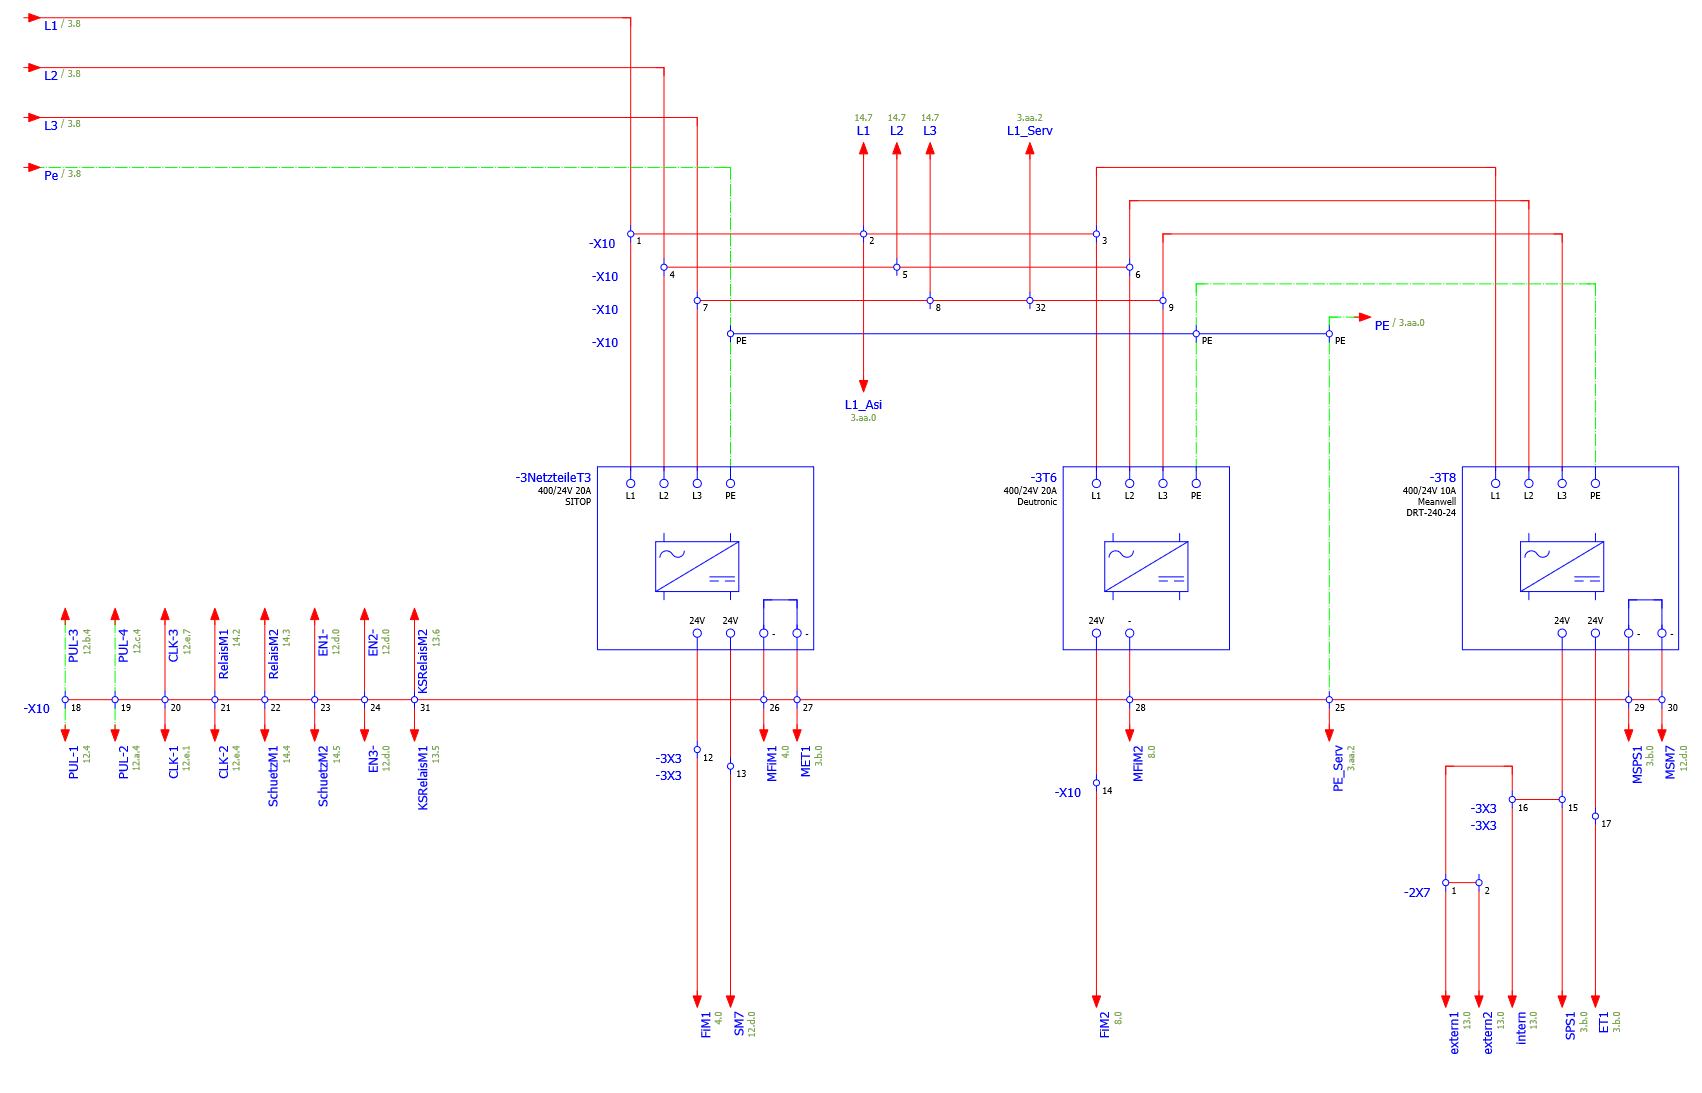
\includegraphics[width=0.9\textwidth]{Vogis Bilder/Netzteile_Schaltplan.png}
        \caption{Schaltplan: Netzteile}
        \label{fig:Netzteile}
    \end{figure}
    Zwei der Netzteile (Deutronic und SITOP) können jeweils 20A auf der 24V-Seite liefern. Diese leistungsstarke Versorgung wird verwendet, um die Schrittmotoren zu versorgen. Beide Gleichrichter-Netzteile teilen sich die Schrittmotoren auf. Drei auf die Deutronic und vier auf die SITOP. Von der SITOP kommen zwei 24V Ausgänge. Das eine Netzteil ist mit einem von zwei Feed-In-Modulen verbunden. Der Zweite ist direkt mit einem ungesicherten und kleineren Schrittmotor verbunden. Die Deutronic bietet einen Ausgang, dieser ist mit dem zweiten Feed-In-Modul verbunden. Damit ist auf dieser Seite die Versorgung von den Schrittmotoren gewährleistet. Übrig bleibt noch das Netzteil von der Firma Meanwell. Dieses ist mit 10A leistungsschwächer. Dieses Netzteil wird nur zur Versorgung von den Logikkreisen verwendet, darum wird nicht mehr Leistung benötigt. Das bedeutet, von den beiden 24V DC Ausgängen dieses Netzteils sind Verbindungen zur SPS, ET200 und internen sowie externen Not-Aus Schaltern gezeichnent. Auf dieser Seite bedeutet dies Klemmen mit Abgängen.\\    
    Die 24V-DC-Minuspole der Netzteile sind auf Reihenklemmen geführt. Diese Reihenklemmen sind über Querverbinder miteinander verbunden und im Anschluss auch mit den PE-Klemmen der 230V Seite verbunden. Die Entscheidung den Steuerstromkreis zu Erden beruht auf der Norm EN60204-1. Demnach hilft die Erdung gegen EMV-Probleme und gewährleistet im Fehlerfall die Abschaltung (vgl. \cite{elektronet_steuerstromkreis_geerdet} u. \cite{beckhoff_steuerstromkreis_geerdet}).
    \paragraph{ASi-Versorgung sowie Service-Schnittstelle}\mbox{}\\
    Der folgende Abschnitt ist ein Nachtrag, denn anfänglich wurde nicht bedacht, dass der ASi-Kreis eine eigene 24V-DC-ASi-Versorgung braucht. Auf die zweite Seite ist demnach die ASi-Versorgung gezeichnet sowie der Anschluss an den ET200-ASi-Master. Eingehend sind auf dieser Seite der L1, N und ein Set, Letzteres ist ein Eingang beim ASi-Master und wird von der SPS aus gesetzt und ausgehend ist der ASi-BUS vom ASi-Master. Weiters befindet sich auf dieser Seite auch die Verdrahtung der Service-Schnittstelle. Diese wird auch zusätzlich mit einem zweiphasigen Leitungsschutzschalter gesichert.
    \paragraph{Versorgung der Logik}\mbox{}\\
    Auf der dritten Seite ist der Versorgungsanschluss von SPS und ET200 gezeichnet. Eingehend sind 24V einmal für die SPS sowie für die ET200 und der jeweilige Minuspol dazu. Auf dieser Seite sind Drahtverbindungen gezeichnet, die die SPS, die Ein und Ausgangskarten sowie die beiden PTO-Karten versorgen.
    \paragraph{Versorgung von DC-Sicherungen}\mbox{}\\
    Auf der vierten Seite findet sich das erste Feed-In-Modul von Weidmüller. Hier eingehend sind 24V, mit Minuspol, von der SITOP und ausgehend sind die Brückenverbindungen von den DC-Sicherungen. Das wären zwei mal Brücken für 24V, zwei mal Brücken für GND und eine Brücke für den BUS dieser Baugruppe.
    \paragraph{DC-Sicherungen 8 A}\mbox{}\\
    Auf den nächsten beiden Seiten finden sich jweils eine 8A-DC-Sicherung. Eingehend sind die bereits genannten Brücken, diese gehen dann auch weiter zur nächsten Sicherung, und ausgehend sind einmal + und - für die stärkeren Schrittmotoren.
    \paragraph{DC-Sicherung 2 A}\mbox{}\\
    Auf Seite sieben findet sich eine 2A-DC-Sicherung für einen von drei schwächeren Schrittmotoren. Diese hat ebenfalls die Brückenverbindung eingehend, allerdings hört die Brückenverbindung mit dieser Sicherung auf. Das bedeutet ein Feed-In-Modul versorgt drei Sicherungen. Abgehend hat diese Sicherung + und - für den passenden Schrittmotor.
    \paragraph{Zweiter DC-Sicherungsblock}\mbox{}\\
    Ab der achten Seite wiederholen sich die letzten vier Seiten, mit dem Unterschied, dass die gebrückte Versorgungsleitung nicht von der SITOP kommt, sondern von der Deutronic. Auf der Ersten ist damit wieder das Feed-In-Modul für die zweite Baugruppe. Somit hat man auf den drei folgenden Seiten drei DC-Sicherungen (8A, 8A, 2A), auf jeder Seite jeweils eine und von jeder Sicherung zwei Abgänge für die passenden Schrittmotoren.
    \paragraph{2 Nm Schrittmotor mit zugehörigem Treiber}\mbox{}\\
    Wenn wir diesen Teil des Schaltplanes von der Motorseite aus betrachten, gibt es für den Motor vier Spulenanschlüsse (zwei pro Spule), die in Tabelle \ref{tab:motoranschluesse} aufgelistet sind.
    \begin{table}[H]
        \centering
        \begin{tabular}{|c|c|c|c|}
            \hline
            \textbf{A+} & \textbf{A-} & \textbf{B+} & \textbf{B-} \\ \hline
        \end{tabular}
        \caption{Anschlüsse des Schrittmotors}
        \label{tab:motoranschluesse}
    \end{table}
    Im Vergleich zum Motor hat der über eine Welle gekoppelte Geber mehr Kontakte, diese sind in Tabelle \ref{tab:geberanschluesse} aufgelistet.
    \begin{table}[H]
        \centering
        \begin{tabular}{|c|c|c|c|c|c|}
            \hline
            \textbf{EB+} & \textbf{EB-} & \textbf{EA+} & \textbf{EA-} & \textbf{VCC} & \textbf{GND} \\ \hline
        \end{tabular}
        \caption{Anschlüsse des Gebers}
        \label{tab:geberanschluesse}
    \end{table}
    Der Treiber CL57C hat Ausgänge, die genau dieselbe Bezeichnung haben. Die gleichnamigen Anschlüsse wurden miteinander verbunden. \\\\
    Da der Motor nicht im Schaltschrank sondern am Lagerregal verbaut wird, muss vom Treiber zum Motor beziehungsweise Geber ein Kabel verlegt werden. Dies wiederum bedeuet, dass im Schaltschrank vom Treiber zuerst auf Reihenklemmen gegenagen wird und an diese Reihenklemmen dann die Kabel geklemmt werden. Für den Schrittmotor wird ein 5 adriges Kabel (inklusive PE) verwendet mit der Kabelbezeichnung \enquote{ÖLFLEX® CLASSIC FD 810 CY 5G0,75}. Der PE Leiter wird an eine Erdung angeklemmt und dieses Kabel hat, um die elektromagnetische Verträglichkeit zu gewährleisten, eine Schirmung. Die Schirmung muss, um zu funktionieren, an die Erdung gelegt werden, weil der Schirm nur so eine Senke sein kann, für die von den Leitern abgestrahlten elektromagnetischen Wellen. Das Kabel wird auf einer Ankerschiene mit der entsprechenden Zugentlastungsklemme, auf dem Erdungsmodul, nicht nur zugentlastet, es wird auch der Schirm geerdet. Dabei muss dann bedacht werden, dass die Klemme Kontakt zum Schirm hat, und die Ankerschiene geerdet sein muss. Der Schirm sowie die Erdung dessen wurde im Schaltplan hinzugefügt.\\    
    \begin{figure}[h]
        \centering
        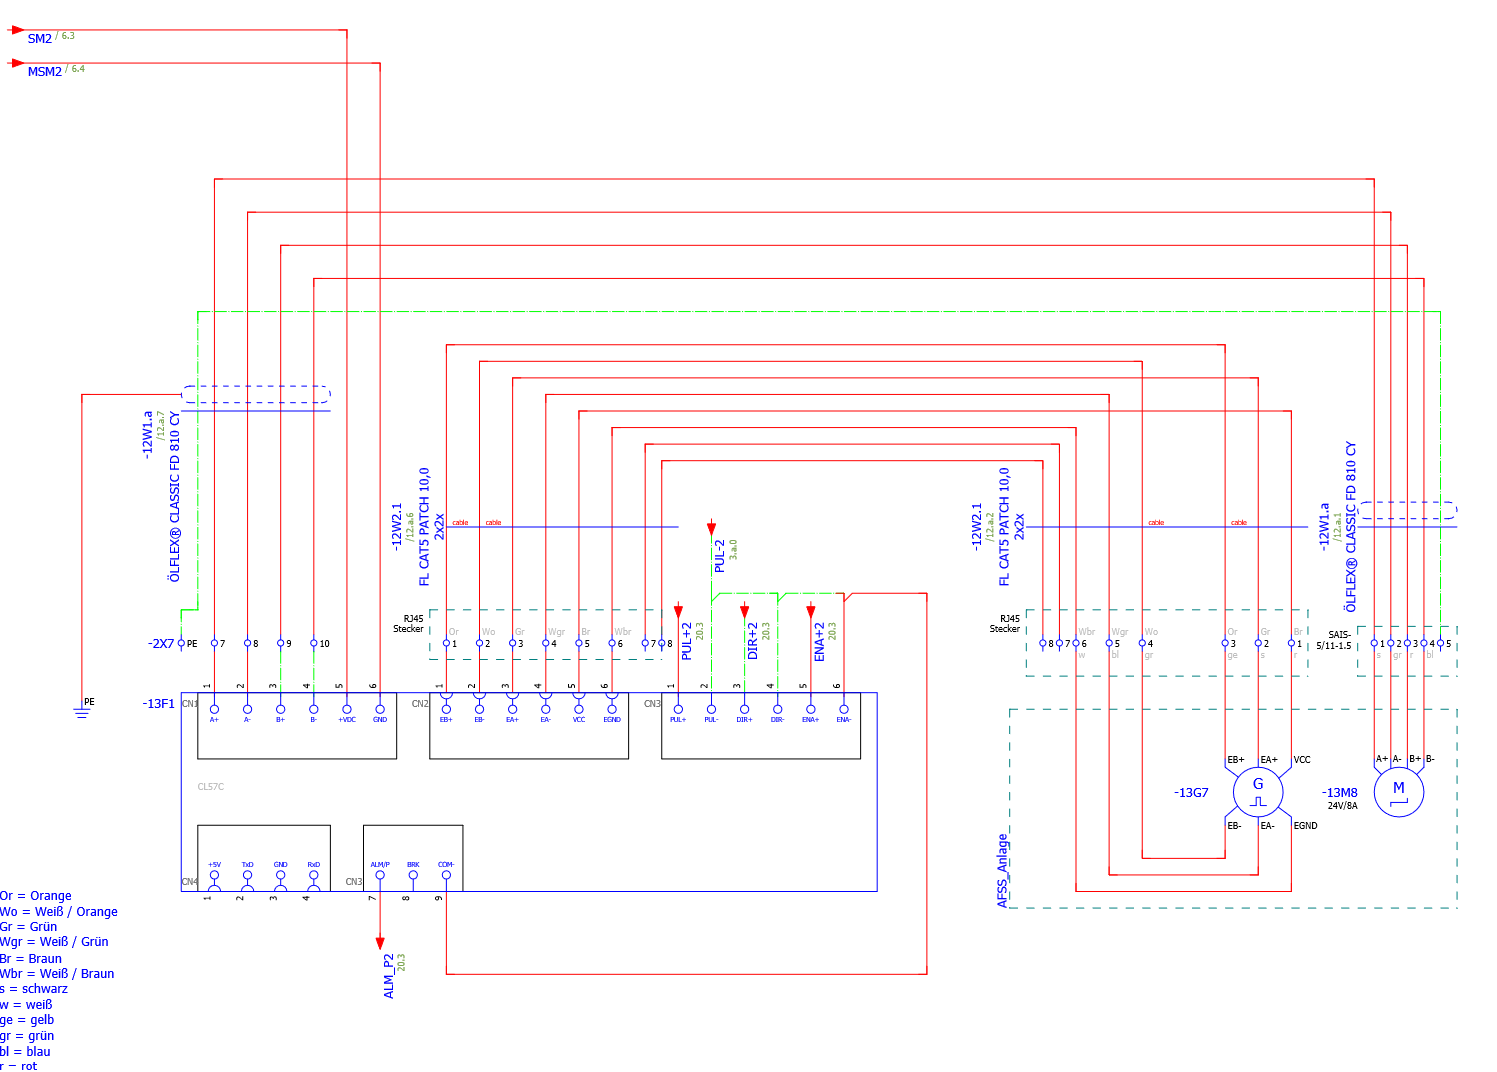
\includegraphics[width=0.9\textwidth]{Vogis Bilder/Schaltplan_SM1.png}
        \caption{Seite 13 des Schaltplans, SM ohne Bremse}
        \label{fig:SMohneBremse}
    \end{figure}
    Bezüglich den Motorkabeln wurde ebenfalls die Farbe der Adern bedacht. Während beim \enquote{ÖLFLEX® CLASSIC FD 810 CY 5G0,75} die Adern durchgängig nummeriert sind, sind es die Adern des Schrittmotors nicht. Diese haben die Farben Schwarz, Grün, Rot und Blau. Da man beim Verdrahten nicht immer wissen kann, welche Farbe zu welchem Anschluss führt, wurde auch dies im Schaltplan festgehalten (vgl.\cite{Nema_SM_Kontaktbezeichnung}).\\
    Auch der Geber benötigt ein Kabel. Für diesen wurde auf Patch-Kabel gesetzt. Das achtadrige \enquote{FL CAT5 PATCH 10,0} bietet die Möglichkeit RJ45 Stecker zu verwenden. Diese befinden sich jeweils an den Enden des Kabels und ersparen im Schaltschrank eine Menge Reihenklemmen, da man nur für die Buchse eine Aussparung bedenken muss. Vor allem im Entwicklungsprozess ist das komfortable An- und Abstecken ein großer Vorteil. Aber auch im späteren Normalbetrieb ist es von Vorteil, bei zum Beispiel einer Umsiedelung des AFSS, die Kabel einfach abstecken zu können. Auch diese Kabel haben einen Schrim, der über den RJ45 Stecker geerdet werden kann.\\\\
    Damit wäre die Kommunikation von Treiber, Motor und Geber gezeichent. Doch es gehört auch die Kommunikation zur SPS dazu. Die Kontakte des Treibers für die Kommunikation mit der SPS sind in der Tabelle \ref{tab:anschluesse} aufgelistet.\\ 
    \begin{table}[H]
        \centering
        \begin{tabular}{|c|c|c|c|c|c|c|c|c|}
            \hline
            \textbf{PUL+} & \textbf{PUL-} & \textbf{DIR+} & \textbf{DIR-} & \textbf{ENA+} & \textbf{ENA-} & \textbf{ALM} & \textbf{BRK} & \textbf{COM-} \\ \hline
        \end{tabular}
        \caption{Übersicht der Anschlüsse}
        \label{tab:anschluesse}
    \end{table}
    Alle Anschlüsse mit einem \enquote{-} am Ende beschreiben den Minuspol zum jeweiligen Gegenstück mit \enquote{+}. Da in unserem Fall alle \enquote{+} Kontakte von der selben SPS kommen und damit alle die selbe Spannung referenzieren, können PUL-, DIR-, ENA- und COM- zusammengeschlossen werden und daraufhin zur Sammelschiene der Minuspole geklemmt werden.\\
    PUL+ steht für \enquote{pulse} und reguliert die Geschwindigkeit der Drehung,  DIR+ steht für \enquote{direction} und reguliert die Drehrichtung, ENA+ steht für \enquote{enable} und entsperrt den Treiber beziehungsweise gibt frei, dass eine Ansteuerung gewünscht ist. BRK steht für \enquote{break} und würde benötigt werden, wenn eine Bremse angedacht wäre, was in diesem Fall aber nicht der Fall war. ALM steht für \enquote{alarm} und ist ein Ausgang, der einen erkannten Fehler meldet.\\
    ALM wurde mit der Eingangskarte verbunden und PUL+, DIR+ und ENA+ wurden an die zugehörigen Kontakte bei den PTO Karten der SPS gezeichnet. Die vollständige Seite ist auf der Abbildung \ref{fig:SMohneBremse}\\     
    \begin{figure}[h]
        \centering
        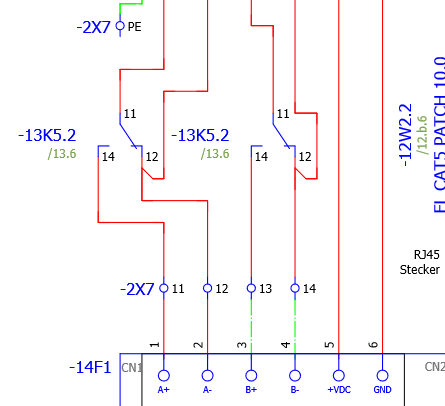
\includegraphics[width=0.5\textwidth]{Vogis Bilder/Schaltplan_SM_bremse.png}
        \caption{Zusätzliche Kurzschließung von Spulen bei horizontalen Antrieben}
        \label{fig:SMmitBremse}
    \end{figure}
    Während die ersten beiden SM-Treiber Schrittmotoren ansteuern, die keine Bremsfunktion brauchen, da sie den Apparat nur horizontal bewegen und damit bei plötzlichem Ausfall, die Anlage auf dieser Achse zum Stillstand kommt, brauchen die anderen zwei Motoren eine Bremsfunktion. Die zwei restlichen SM-Treiber steuern Motoren an, die zum Heben des Gabelapparates da sind. Sollten diese unerwartet ausfallen, würde die Schwerkraft das Konstrukt zu Boden fallen lassen. Deswegen sollen im Fehlerfall Relaiskontakte die Spulen der Schrittmotoren kurzschließen und damit eine bremsende Wirkung ermöglichen. Dabei funktioniert das Prinzip so, dass bei plötzlicher Spannungsabwesenheit das Relais loslässt und die Spulen kurzgeschlossen sind und damit eine bremsende Wirkung entsteht. Das heißt im spannungsfreien Zustand sind die Spulen kurzgeschlossen (siehe Abbildung \ref{fig:SMmitBremse}).
    \paragraph{40 Ncm Schrittmotoren mit zugehörigen Treibern sowie Relais}\mbox{}\\
    Auf den darauf folgenden zwei Seiten befindet sich die Steuerung von den schwächeren Schrittmotoren (siehe Abbildung \ref{fig:SMkleine}). Auch diese haben Treiber und Motoren, aber keine Geber.\\
    Auch die Treiber für die schwächeren Schrittmotoren haben einen enable-Eingang. Dieser ist jedoch dann freigegeben, wenn der Eingang spannungsfrei ist. Aufgrund dieser Eigenschaft besteht die Gefahr, dass die Schrittmotoren losfahren, bevor die SPS die Spannung aufgebaut hat, die die Motoren dann steuern würde. Beispielsweise wenn die Anlage einen Neustart durchführt, könnte diese Situation entstehen. Darum werden die Eingänge \enquote{invertiert}. Ein Relaiskontakt, ein Öffner, setzt den EN-Eingang immer auf 24V, erst sobald die SPS das Relais ansteuert, kann der Treiber freigegeben werden. Bei drei Treibern erfordert dies drei Relais. Auf Seite 17 befinden sich somit die Relais und deren Öffnerkontakte. Anfänglich wurden hier fälschlicher weise Schließer eingeplant, im Verlauf der Arbeit wurde diese Entscheidung hinterfragt und demnach auch ausgebessert. Auf der darauf folgenden Seite finden sich die Treiber und Schrittmotoren.\\
    Zu den Treibern kann man sagen, dass alle Treiber ähnlich aufgebaut sind. Wieder gibt es einen Kontakt zur Geschwindigkeitsregelung (CLK+ und CLK-), einen zur Richtungsbestimmung (CW+ und CW-) und den bereits besprochenen Freigabeeingang (EN+ und EN-). Weiters haben die Treiber noch Anschlüsse für die Versorgungsspannung und A+, A-, B+ und B- für die Schrittmotoren. Die Massekontakte werden wieder alle zusammengeschlossen und weitergeführt zur gemeinsamen Masse.\\ 
    Auch für diese Motoren werden die selben Kabel verwendet wie zuvor. Wieder gilt, dass die Schirmung bei der Zugentlastung geerdet wird und auch die Farben der Adern wurden im Schaltplan eingezeichnet.\\
    Auch hier sind die Steuerkontakte von den Treiben an die PTO-Karten der SPS angeschlossen.
    \begin{figure}[H]
        \centering
        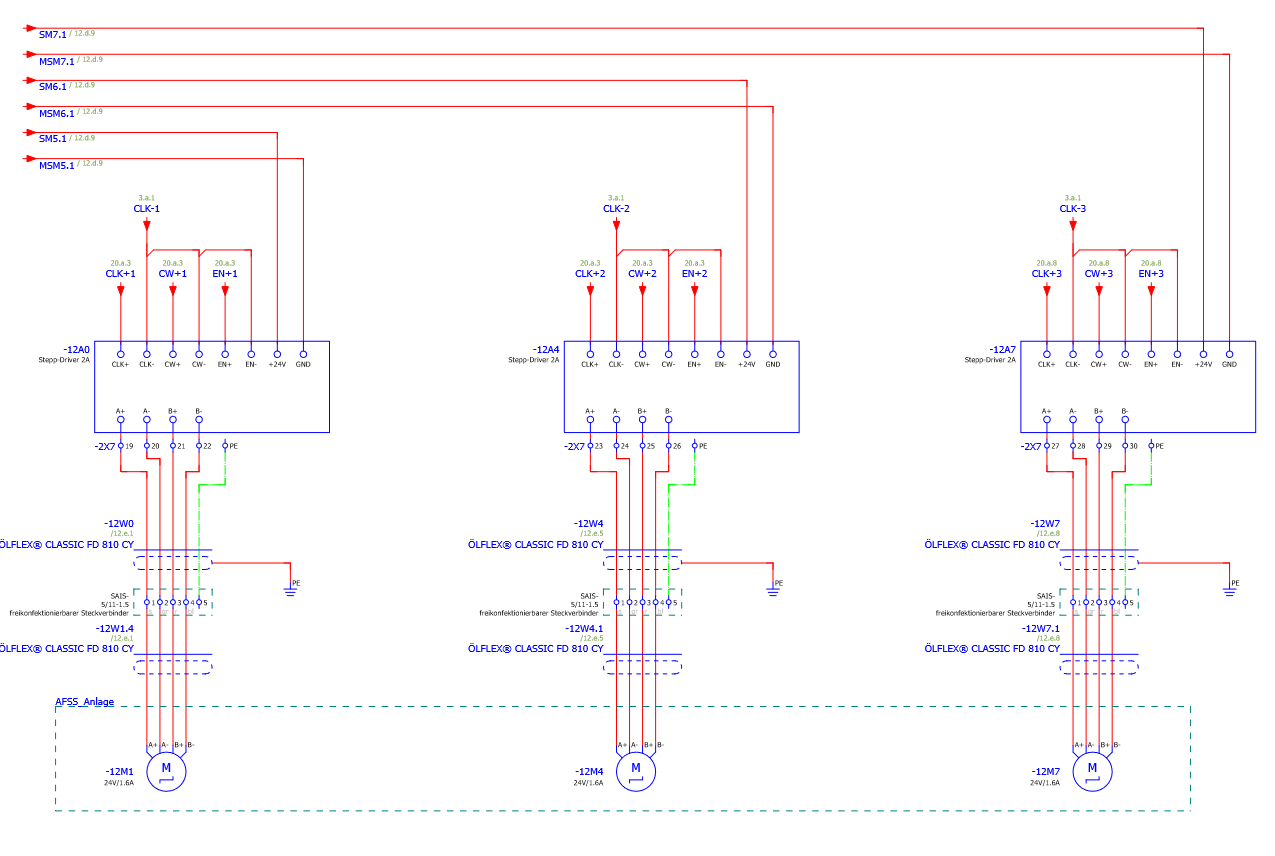
\includegraphics[width=0.9\textwidth]{Vogis Bilder/SM_Klein_Schaltplan.png}
        \caption{40Ncm Schrittmotoren im Schaltplan}
        \label{fig:SMkleine}
    \end{figure}
    \paragraph{Not-Aus, Schlüsselschalter und Relais}\mbox{}\\
    Auf der folgenden Seite befinden sich Not-Aus-Schaltungen und die Relais, die dem Vertikalantrieb die Bremsfunktion geben. In Summe sind es vier Not-Aus und zusätzlich noch der Schlüsselschalter zur Freigabe. Für die fünf Sensoren gibt es drei Versorgungsleitungen. Je nach räumlicher Position teilen sich die Komponenten eine Leitung, und alle haben jeweils einen Abgang zur SPS-Eingangskarte. Die Relais bekommen ihre Versorgung von der SPS und haben Abgänge zur gemeinsamen Masse. Die Funktion der Relais wurde bereits beschrieben.
    \paragraph{Asynchromotor mit Steuerung}\mbox{}\\
    Die nächste Seite zeigt die ganze Steuerung des Asynchromotors, welcher das Förderband antreibt. Hierfür gibt es Schütz, die in einer Wendeschützschaltung den Asynchronmotor ansteuern. Es ist keine Drehzahlregelung nötig. Die Schütze blockieren sich gegenseitig und werden angesteuert über zwei Relais. Diese Relais werden direkt von der SPS angesteuert. Beim Asynchronmotor gibt es noch einen Motorschutzschalter, dessen genauere Auslegung im Verlauf der Diplomarbeit noch genauer beschrieben wird.
    \paragraph{Siemens-PTO-Karten}\mbox{}\\
    Die Seiten 21 und 22 zeigen die PTO-Karten der SPS. PTO steht für Pulse-Train-Output und steuert die Treiber an. Ursprünglich wären für diese Aufgaben PWM-Karten von Weidmüller verwendet worden, es ist allerdings bei Testversuchen aufgefallen, dass diese nicht in der Lage sind, variable Frequenzen zu erzeugen. Damit musste eine Alternative gefunden werden. Die Siemens PTO-Karten sind in der Lage die Frequenzen auch während des Betriebes zu ändern und damit ermöglichen sie sanftes Anfahren der Schrittmotoren. Eine PTO-Karte kann vier Schrittmotoren steuern.\\
    Diese Karten haben mehrere Ausgänge und Eingänge. Im Fall des AFSS gehen vier mal die PUL+ und DIR+ und ENA+ aus und eingehend sind die vier ALM (Alarmmeldungen). Das sind die Kontakte von den vier stärkeren Treibern und damit ist die erste PTO-Karte voll ausgenutzt. Mit der zweiten PTO-Karte werden die drei schwächeren Treiber angesteuert. Diesesmal wieder mit den unterschiedlich benannten Kontakten.
    \paragraph{Siemens-DI-Karten}\mbox{}\\
    Auf der folgenden Seite befindet sich die Eingangskarte der SPS mit den Eingängen. Dabei werden primär die Zustände der Not-Aus-Schalter abgefragt und die des Schlüsselschalters.
    \paragraph{Siemens-DO-Karten}\mbox{}\\
    Auf Seite 24 befindet sich die Ausgangskarte der Siemens SPS. Mit dieser werden ausschließlich nur Relais angesteuert. Diese sind für die Invertierung der Enable-Eingänge der Treiber zuständig, für das Steuern der Schütze für den Asynchronmotor und zuletzt auch für die Bremsfunktion. Damit ist die Schaltung zur Steuerung aller Schrittmotoren fertig. Auf den folgenden Seiten wurde dann die Schaltung der ASi-Sensoren gezeichnet
    \paragraph{ASi-Slaves und Sensoren}\mbox{}\\
    Bezüglich dem ASi-Netz ist zu wiederholen, dass der ASi-Master mit den Slaves über einen zweiadrigen ASi-Bus kommuniziert. Für diesen Bus gibt es ein eigenes Kabel, aber da mit dem Material gearbeitet werden muss, was vorhanden ist, wird beim AFSS das selbe fünf adrige Ölflex verwendet wie für die Motoren. In diesem ungünstigen Fall werden von den fünf Adern am Ende nur zwei verwendet.\\
    \begin{figure}[H]
        \centering
        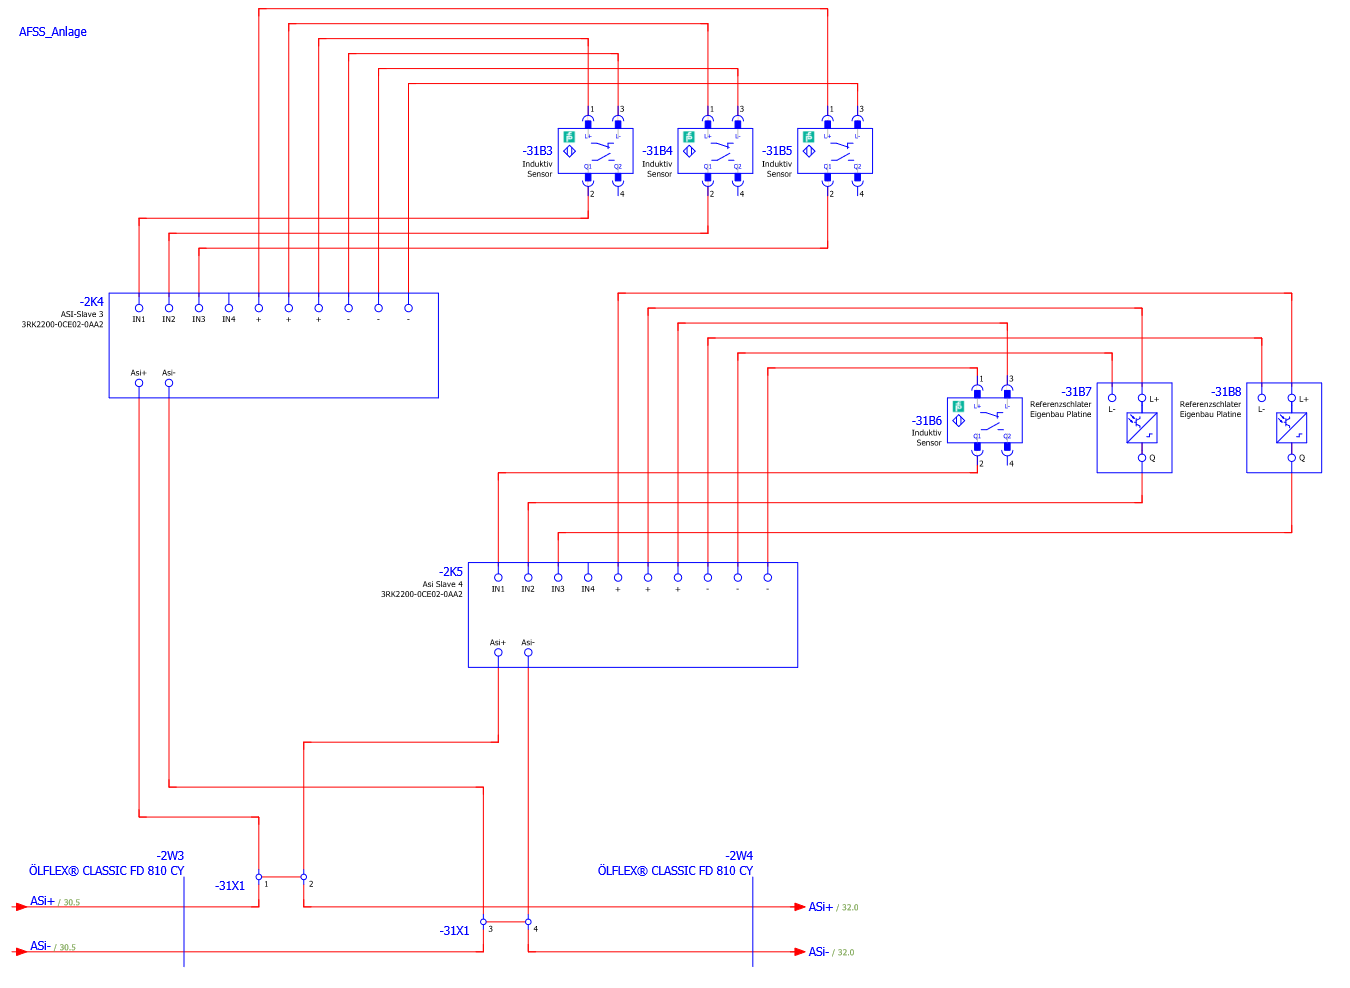
\includegraphics[width=0.9\textwidth]{Vogis Bilder/ASI_Schaltplan_sensoren.png}
        \caption{Sensoren mit den ASi-Slaves, erste Seite von vier}
        \label{fig:ASI_Sensoren}
    \end{figure}
    Bezüglich den Slaves ist festzuhalten, dass ursprünglich ein Slave mit sieben Inputs geplant war. Dieser wäre in der Schule auch ausreichend vorhanden gewesen. Allerdings ist es bei den Testläufen nicht gelungen, eine Kommunikation zwischen diesen Slaves und dem Siemens ASi-Master herzustellen. Deswegen werden anstatt vier Slaves mit sieben Eingängen, nun sieben ASi-Slaves von Siemens mit jeweils vier Eingängen verwendet. Der genaue Typ ist 3RK2200-0CE02-0AA2 und es ist möglich mit diesem zu kommunizieren.\\
    Der Bus fährt auf mit Steckverbindern verbundene Reihenklemmen, von dort dann auf die jeweiligen Slaves. Es sind immer zwei Slaves zusammen und werden gemeinsam mit Reihenklemmen auf dem AFSS auf Hutschienen montiert. Wie die Sensoren mit den ASi-Slaves verbunden sind, sieht man auf der Abbildung \ref{fig:ASI_Sensoren} und für eine genaue Erklärung zu den Sensoren siehe Kapitel \ref{sec:Sensorik}.\\
    In Summe erstreckt sich der genaue Schaltplan der ASi-Slaves über die letzten vier Seiten.
    \paragraph{Topologieansichten}\mbox{}\\
    Nachdem alle Seiten gezeichnet und überarbeitet wurden, wurden für den ASi-Bus und den PROFIBUS noch passende Topologieansichten gezeichnet. Diese bieten eine übersichtliche Darstellung der Busse.
    \paragraph{Übersichtsblätter}\mbox{}\\
    Daraufhin wurden noch zwei Übersichtsblätter gezeichnet. Auf diesen ist die gewünschte Anreihung der Siemens SPS und ihren Karten sowie die der ET200 mit ihrem ASi-Master.
\subsection{Die Auslegung diverser Schaltschrankkomponeten}
    \paragraph{Fehlerstomschutzschalter}\mbox{}\\
    Der FI ist ein Schutzorgan, welches im Fehlerfall den Stromkreis unterbricht. Dieser erkennt wenn der Summenstrom von L1, L2, L3 und N nicht mehr gleich Null ist und schaltet dann ab.\\
    Beim FI gibt es verschiedenste Arten. Die Älteste wäre der TYP AC, es gibt aber auch noch TYP A, B und F sowie weitere. Von den genannten Typen wurde für das AFSS ein Fehlerstromschutzschalter der Variante A gewählt, da bei dieser Anlage das Erkennen von Wechselströmen und Pulsströmen genügt. Das liegt daran, dass kein Spezialfall vorliegt, der einen anderen Typen erfordern würde (vgl. \cite{FI-Typen}).
    \paragraph{Leitungsschutzschalter}\mbox{}\\
    Bei der Auswahl des Leitungsschutzschalters ist die Schaltcharakteristik sowie der Bemessungsstrom zu berücksichtigen. Da im AFSS die ASM zu hohen Anlaufströmen führt, wurde eine Charakteristik des Typs C gewählt, dieser ist anzuwenden in Schaltkreisen mit Motoren oder Handwerkzeug (vgl. \cite{SeyrRösch}, S. 100–110). Für den Bemessungsstrom wurde 13 A ausgewählt, da dieser Wert der nächsthöhere zum Nennstrom war. Der Nennstrom wurde ermittelt aus der Summe der einzelnen Nennströme der Verbraucher multipliziert mit einem Gleichzeitigkeitsfaktor. Bei letzterem Faktor wurde geschätzt wie viele Verbraucher gleichzeitig laufen werden. Die Gabel-Antriebe beispielsweise werden nie gleichzeitig zu irgendeinem anderem Motor ein oder ausfahren. 
    \paragraph{Motorschutzschalter}\mbox{}\\
    Der Asynchromotor hat im Falle des AFSS einen Nennstrom von 1,9 A. Beim AFSS wird ein Standardmotorschutzschalter verwendet, der auf den Nennstrom des Motors angepasst wurde. 
    \paragraph{Leiterquerschnitte}\mbox{}\\
    Der Leiterquerschnitt ist abhängig vom Spannungsabfall, der aufgrund von kurzen Längen im Schaltschrank vernachlässigbar ist, von Verlegeart und Nennstrom. Der Leiterquerschnitt hängt auch immer mit den Sicherungselementen zusammen, da der Leiter so lange den Strömen standhalten muss, bis das Schutzelement auslöst. Deswegen wird im AFSS ein Leiterquerschnitt von 2,5 mm² verwendet, bis zu entsprechenden Sicherheitselementen und von dort aus wird dann auf 0,75 mm² reduziert (vgl. \cite{SeyrRösch}, S. 100–110).\\ 
    Alle Erdungskontakte sind mit 2,5 mm² verdrahtet um alle potentiellen Fehlerströme auszuhalten.\\
    Die Farben der einzelnen Drähte entsprechen dem schulinternen Standard.
\subsection{Realisierung}
    Wie das Geplante genau umgesetzt wurde wird nun näher beleuchtet.
    \paragraph{Rädermontage}\mbox{}\\
    Der erste Schritt vom Serverschrank zum Schaltschrank des AFSS war die Mobilmachung. Dem Serverschrank wurden vier Räder in den unteren Ecken hinzugefügt. Dafür wurden in den bestehenden Boden für jedes Rad vier Löcher manuell gebohrt. Die Räder wurden daraufhin mit Schrauben, Beilagscheiben und Muttern montiert.\\
    Bei den Rädern handelt es sich um zwei fixierte und zwei sich um 360° drehende Räder. Die Räder wurden paarweise nebeneinader angeordnet (siehe Abbildung \ref{fig:Raeder_montiert}).
    \begin{figure}[h]
        \centering
        \includegraphics[width=0.6\textwidth]{Vogis Bilder/Räder.jpg}
        \caption{Montierte Räder am Schaltschrank}
        \label{fig:Raeder_montiert}
    \end{figure}
    \paragraph{Filou-NC}\mbox{}\\
    Nachdem die Module in AutoCAD neugezeichnet (siehe Abschnitt \ref{AutoCAD}) wurden, konnten die DXF-Dateien in Filou-NC importiert werden.\\
    In Filou-NC wurde die gesammte DXF-Datei importiert. Danach konnte man unerwünschte Teile der Zeichnung löschen, wenn beispielsweise mehrere Module in der selben Zeichnung vorhanden waren, mussten die, die nicht gefräst werden sollten, gelöscht werden. Daraufhin wurde die Zeichnung noch bereinigt, das heißt, dass doppelte Linien gelöscht wurden. Das Programm liefert hierfür ein fertiges Tool. Gewisse Längen der Zeichnung mussten nun noch unterbrochen werden. Das diente dazu, dass beim Fräsvorgang die Platte immer zumindest an den Unterbrechungen mit der ursprünglichen Platte verbunden blieb. Verhindert wird, dass sich die Platte verschiebt und somit nicht mehr an den richtigen Stellen gefräst wurde.\\
    Nachdem die DXF-Zeichnung vorbereitet war, musste nun der Fräsablauf programmiert werden. Dazu musste im Programm dem Ablauf ein Startpunkt gegeben und der Nullpunkt der Zeichnung gesetzt werden. Daraufhin konnte man das \enquote{in Echt} eingespannte Werkzeug auch digital im Programm einfügen, damit das Programm wusste, wie groß der Durchmesser des Werkzeuges war und wie die Spitze des Werkzeuges aussah. Nachdem das Werkzeug eingefügt wurde, war die Sprühdüse, zur Kühlung, einzuschalten und daraufhin konnte man die Konturen der Zeichnung mit dem Werkzeug abfahren. Beim Festlegen der Fräsbahnen war darauf zu achten, dass die richtige Anzahl an Zustellungen eingestellt war. Zustellungen legen fest, dass nicht die ganze Dicke des Materials auf einmal abgetragen wird. Bei dickerem Material ist dies nötig, um das Werkzeug zu schützen.\\
    Wenn diese Schritte erfolgreich ausgeführt wurden, konnte ein NC-Code exportiert werden. 
    \paragraph{Fräsen}\mbox{}\\
    Der genannte NC-Code konnte nun auf die CNC-Fräse geladen werden. Bei der Fräse waren nun noch der Nullpunkt zu setzen und die Werkzeuglänge zu kalibrieren. Bei der Nullpunktsetzung war es wichtig zu beachten, dass keines der Spannelemente, die die Platte auf den Frästisch fixierten, beim Fräsen im Weg sein würde.\\
    Daraufhin konnte der Fräsvorgang gestartet werden. Währenddessen war zu beachten, dass bei der Sprühdüse genügend Flüssigkeit rauskommt, da dies manuell einzustellen war. Ebenfalls war das Werkzeug auf unerwartete Ereignisse zu prüfen, beispielsweise Rauch oder Dampfbildung.\\ 
    Nach dem gelungenen Fräsvorgang wurde die gesammte Fräse gereinigt und die Platte entnommen.\\
    Im angewandten Fall des AFSS wurde zuerst nur ein Modul gefräst und vollständig fertiggestellt, damit festgestellt werden konnte, ob die Maße stimmen. Das erste Modul passte und danach wurden alle verbleibenden Platten an zwei Tagen gefräst.

    \paragraph{Fräsen-Nachbearbeitung}\mbox{}\\
    Nachdem die Platte von der Fräse genommen wurde, hatte diese viele scharfe Kanten. Diese wurden mit entspechendem Werkzeug entgratet. Rückstände von der Kühlflüssigkeit oder vom Kunststoff beziehungsweise Metallspäne wurden sorgfältig entfernt.
    \paragraph{Module-Fertigstellung}\mbox{}\\
    Die Module mussten nun bestückt werden. Dazu wurden die Profilschienen und Montagekanäle abgelängt und mit M5 Schrauben und Muttern montiert.\\
    Die Elemente, die nicht auf Profilschienen montiert werden, wurden mit den für das jeweilige Element vorgesehenen Schrauben und Muttern montiert.\\
    Auf die genanten Profilschienen (Siemens oder Hutschiene) wurden noch die passenden Elemente aufgesteckt.\\
    Die Platten konnten nun in den Schaltschrank auf die vorhandenen Schienen montiert werden. Diese Schienen mussten zuvor nach innen versetzt werden. 
    \begin{figure}[h]
        \centering
        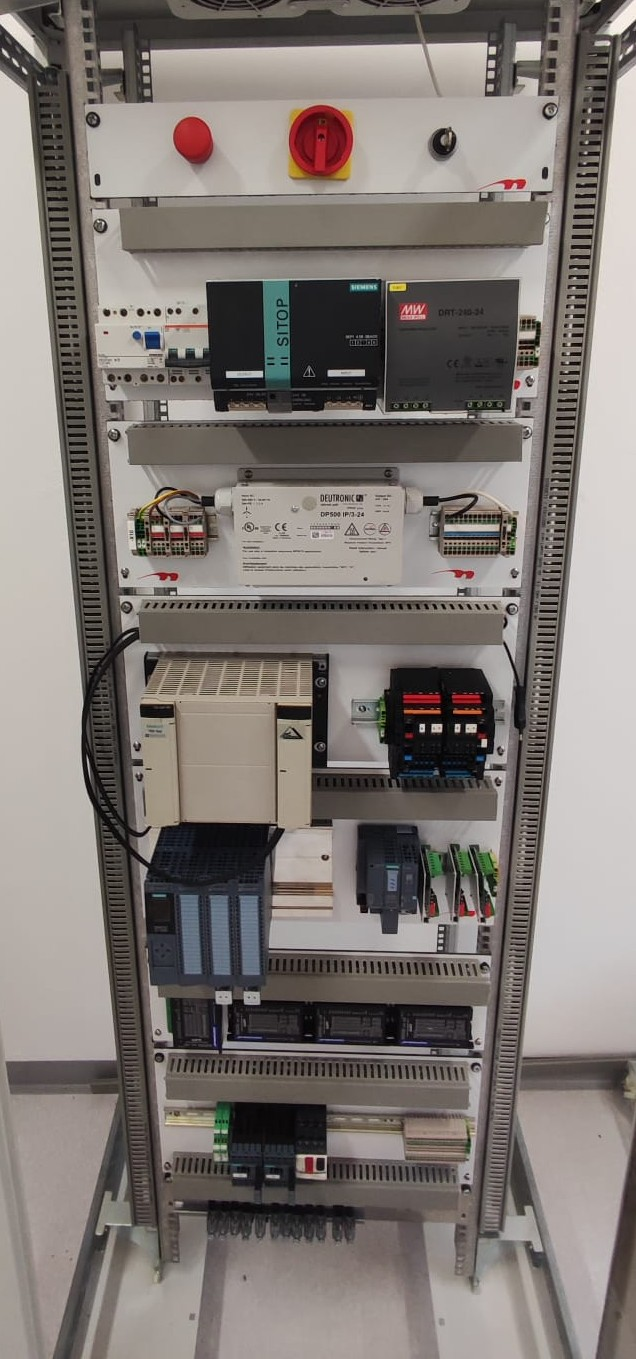
\includegraphics[width=0.3\textwidth]{Vogis Bilder/Schaltschrank_only_module.jpg}
        \caption{Schaltschrank mit eingebauten Modulen}
        \label{fig:Schaltschrank_onlyModule}
    \end{figure}    
    \paragraph{Profilschienen-Verschiebung}\mbox{}\\
    Zwei Profilschienen wurden um ca. 300 mm nach innen versetzt. Dafür wurden die Winkel, die die Profilschienen an den Serverschrank befestigten, gelöst und weiter innen neu montiert. Das war deswegen möglich, da die Winkel an einer weiteren Profilschiene montiert waren. Diese bisher nicht gennante Profilschiene befindet sich im Schaltschrank vier mal und ist oben und unten quer befestigt (siehe Abildung \ref{fig:Clean_Serverschrank}). Nach diesem Schritt konnten die Modulplatten an die verschobenen Profilschienen geschraubt werden (Schaltschrank ohne Verdrahtung siehe Abbildung \ref{fig:Schaltschrank_onlyModule}).  
    \begin{figure}[H]
        \centering
        \begin{subfigure}{0.45\textwidth}
            \centering
            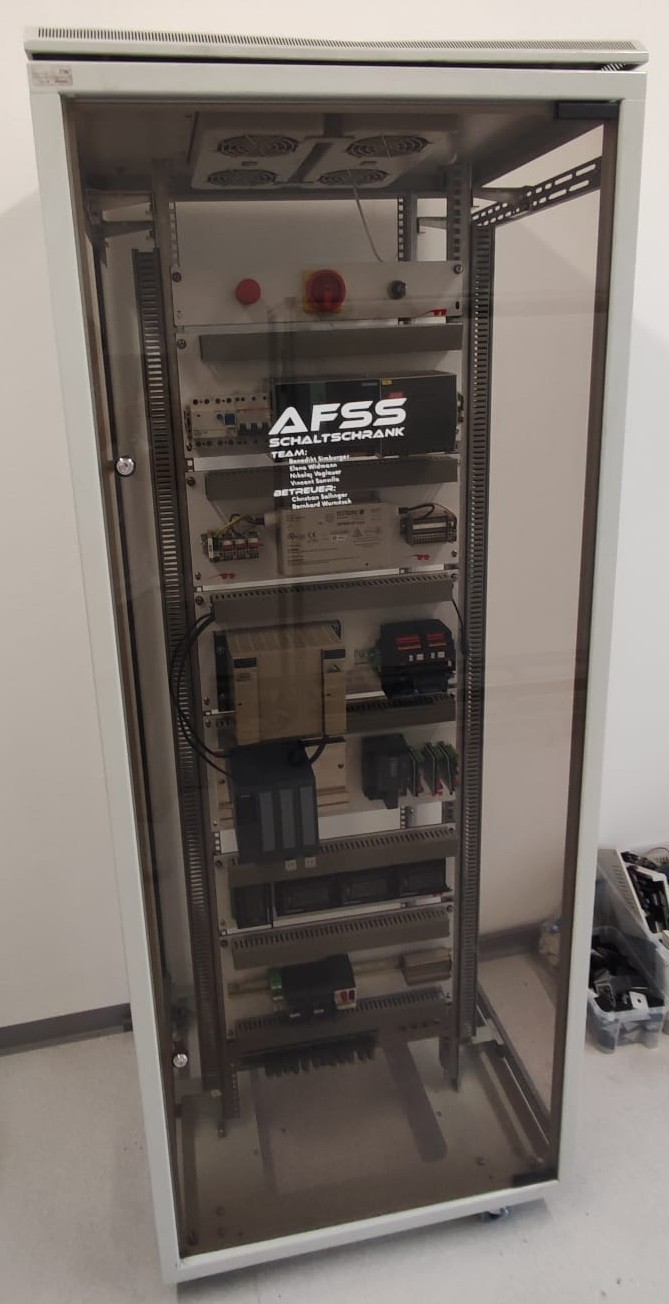
\includegraphics[width=\textwidth]{Vogis Bilder/Schaltschrank_foliert.jpg}
            \caption{Schaltschrank mit Folierung}
            \label{fig:Schaltschrank_foliert}
        \end{subfigure}
        \hfill
        \begin{subfigure}{0.4\textwidth}
            \centering
            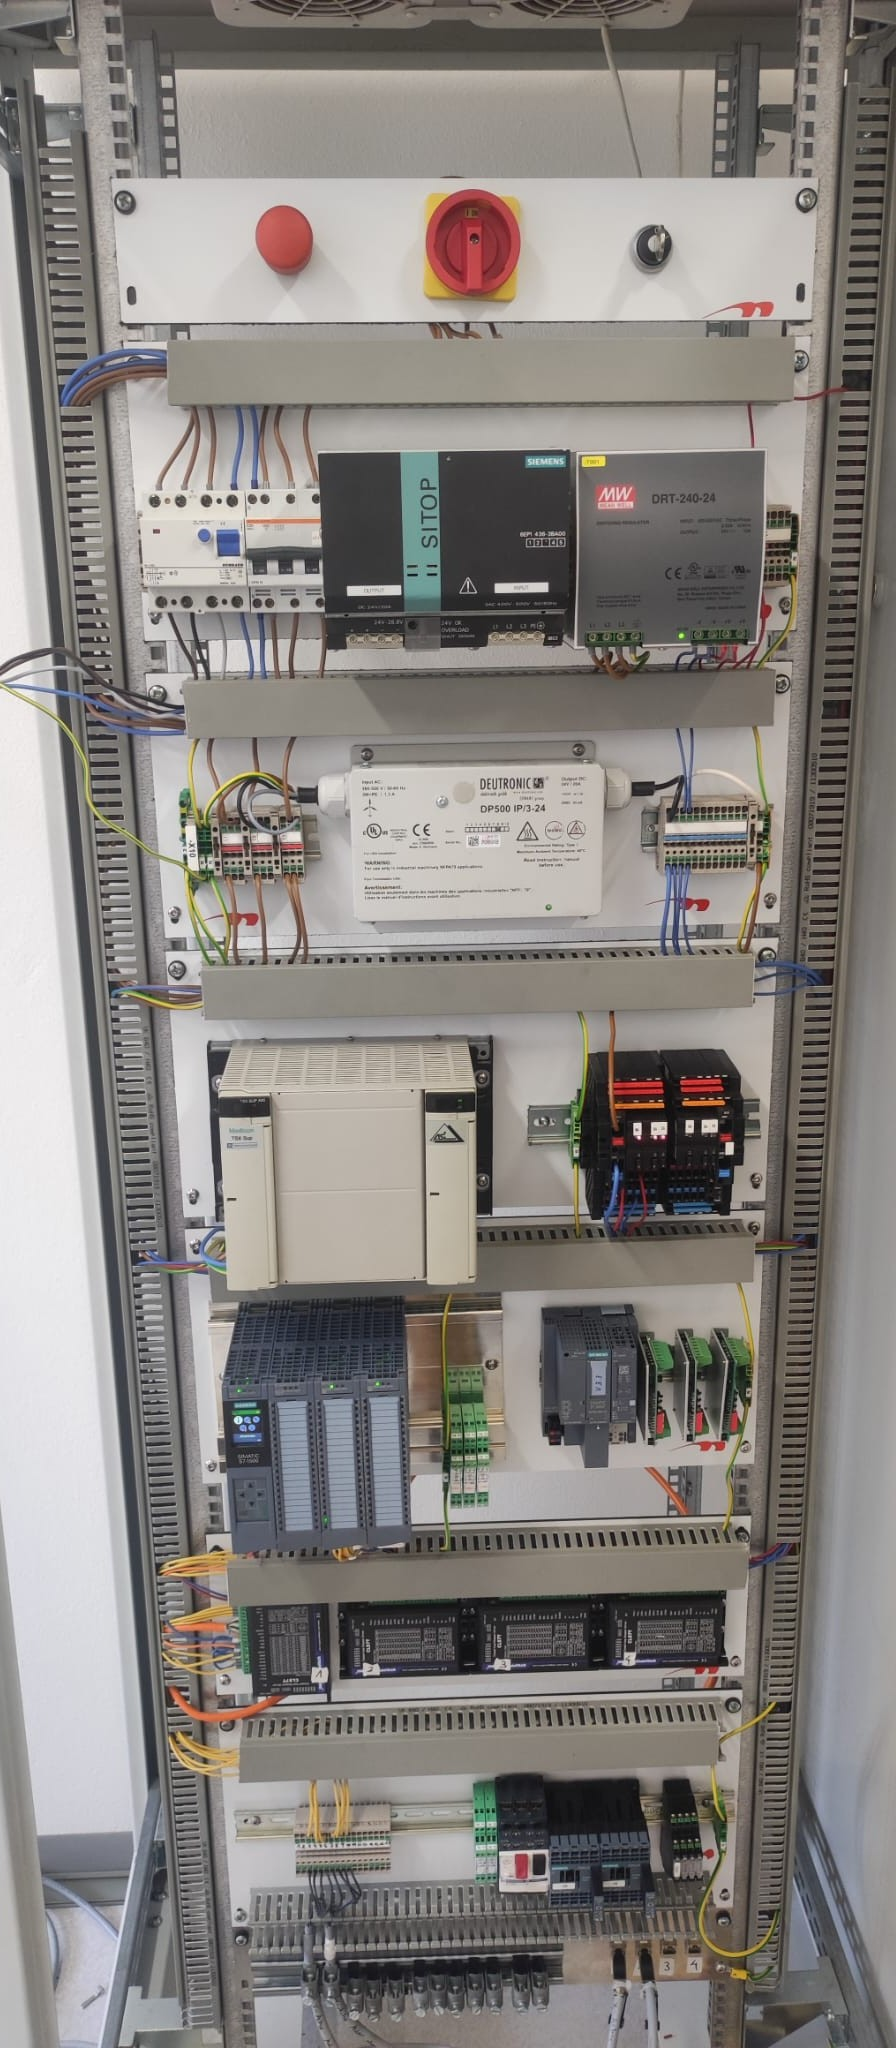
\includegraphics[width=\textwidth]{Vogis Bilder/Schaltschrank_verkabelt.jpg}
            \caption{Schaltschrank mit Verdrahtung}
            \label{fig:Schaltschrank_verkabelt}
        \end{subfigure}
    \end{figure}
    \paragraph{Folierung der Frontscheibe}\mbox{}\\
    Da der Schaltschrank des AFSS mobil ist, wurde entschieden, dass auch für nicht eingeweihte Personen stehts klar sein soll, wessen Schaltschrank dies ist. Dafür wurde der Schaltschrank mit einer Folierung versehen. Auf dieser sind die Teammitglieder aufgelistet, unter anderem FL. Wurnitsch, damit ist die Zugehörigkeit deutlich gekennzeichnet (siehe Abbildung \ref{fig:Schaltschrank_foliert}). Die Folierung wurde mit Hilfe der in der Schule vorhandenen Stickerschneidemaschine erstellt.
    \paragraph{Die Verdrahtung}\mbox{}\\
    Nachdem alle Modifikationen am Serverschrank vollzogen und alle Module eingebaut waren, war die Transformation vom Serverschrank zum Schaltschrank fast vollzogen. Es fehlte noch die Verdrahtung.\\
    Zu dieser ist zu sagen, dass eine vollständige Verdrahtung der ganzen Anlage sich zeitlich nicht ausgegangen. Deswegen wurde ein Kompromiss vereinbart. Dieser besagt, dass genügend verdrahtet wird, sodass die X-Achse ansteuerbar ist (siehe Abbildung \ref{fig:Schaltschrank_verkabelt}).\\
    Beim Verdrahten wurden die bereits genannten Querschnitte beachtet. Auch die schulinterne Leitinie zur Drahtfarbe im Schaltschrank wurde beachtet. Diese besagt: Rot für Versorgungen, Blau für Minus, Gelb für Ausgänge (z.B. SPS), und Orange für Eingänge (z.B. Sensoren).\\
    Beim Verdrahten wird unweigerlich der Schaltplan wieder und wieder durchdacht. Dabei fallen Fehler oder Verbesserungsmöglichkeiten schnell auf. Auch beim Verdrahten des Schaltschrankes des AFSS sind Fehler und Verbesserungspotentialle aufgefallen, beispielsweise, dass die Adern der Encoder-Kabel zwar Farben hatten, diese aber nicht am Schaltplan zugeteilt werden. Ein anderes Beispiel war, dass bei den PTO-Modulen alle Eingänge verschoben waren. Diese und weitere Punkte wurden unverzüglich nachgebessert beziehungsweise hinzugezeichnet.
    \paragraph{Einbau von Service-Schnittstelle}\mbox{}\\ 
    Als letzte Modifikation wurde eine Service-Schnittstelle von Weidmüller in die rechte Metalwand des Schaltschrankes eingebaut (siehe Abbildung \ref{fig:Service_Schnittstelle}). Dazu wurden manuell auf die Seitenwand die erforderlichen Maße angezeichnet. Entlang dieser Markierungen wurde daraufhin, unter Beachtung aller dafür notwendigen Schutzmaßnahmen, mit einem Winkelschleifer geschnitten. Dieser hatte für das Schneiden von Metall dieser Stärke den entsprechenden Aufsatz. 
    \begin{figure}[H]
        \centering
        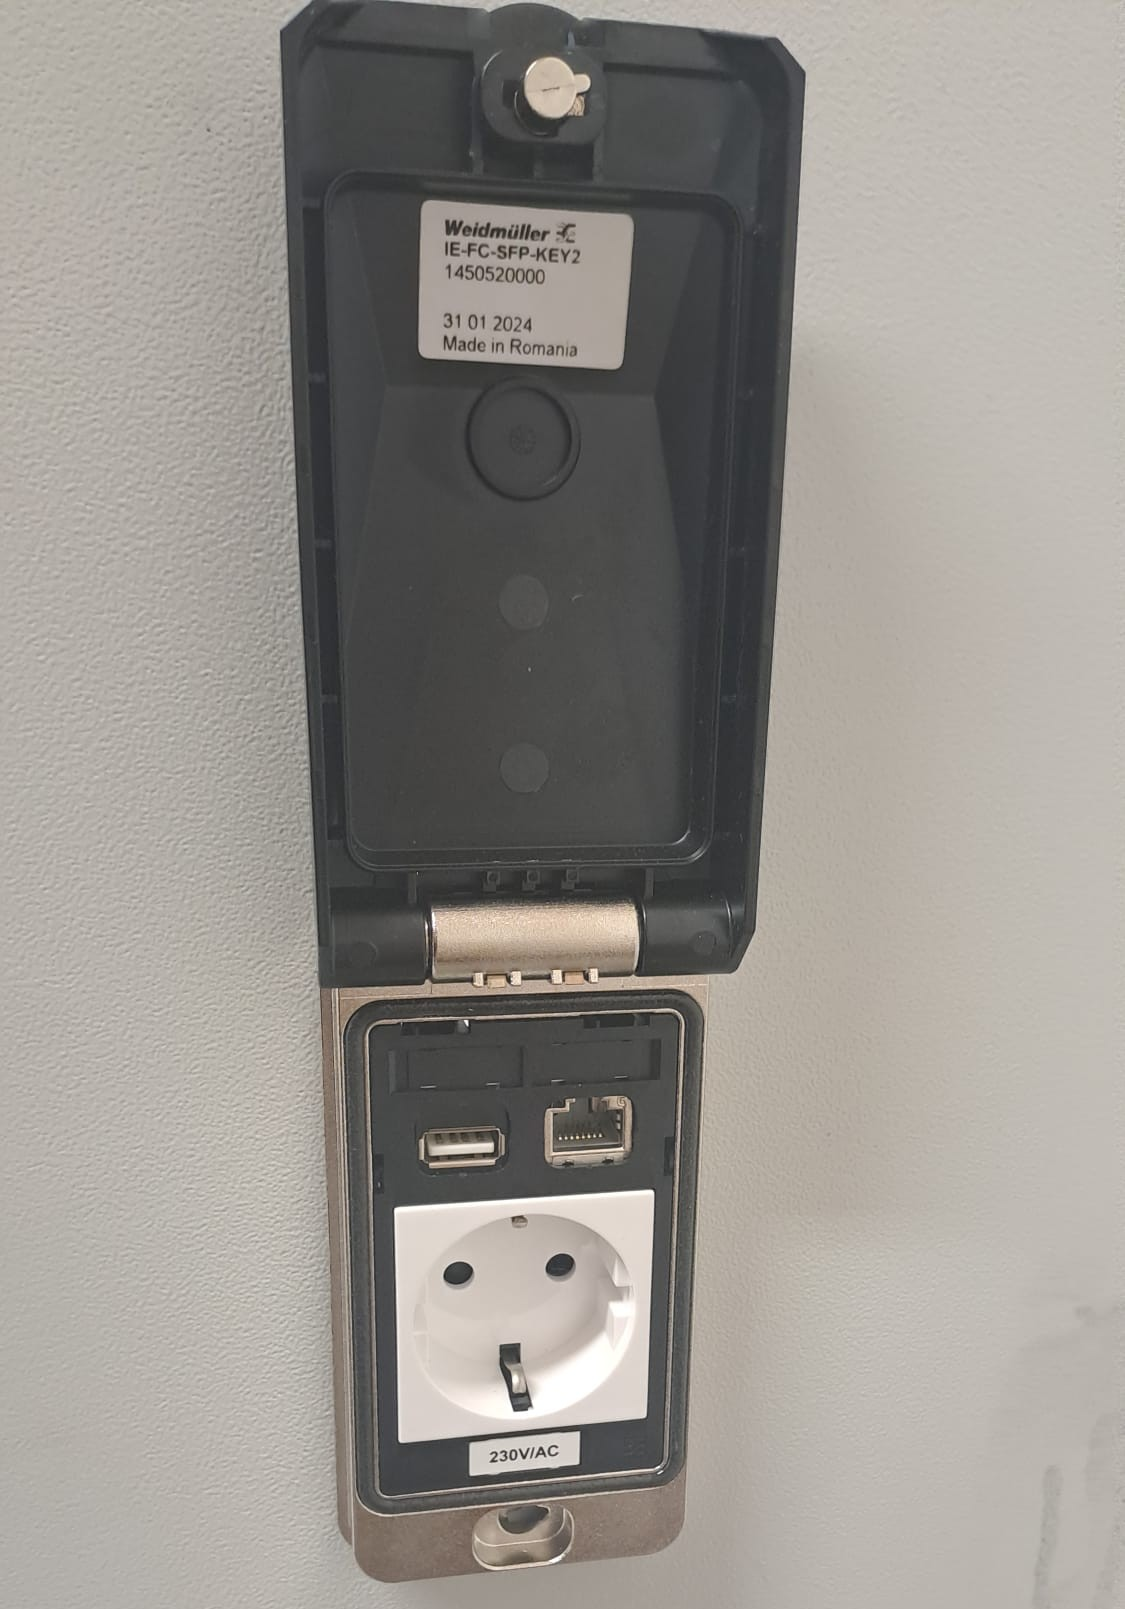
\includegraphics[width=0.4\textwidth]{Vogis Bilder/Service_Schnittstelle.jpg}
        \caption{Service-Schnittstelle von Weidmüller}
        \label{fig:Service_Schnittstelle}
    \end{figure}
\newpage
\subsection{Fazit}\mbox{}
    Die effiziente Realisierung des Schaltschrankes war nur aufgrund einer umfassenden Vorplanung möglich. Das Prinzip des digitalen Zwillings hat sich mehrfach bewehrt und das Erlernte im Bezug auf 3D-Konstruktion ist umfassend.\\
    Der gezeichnete Schaltplan, im Programm E-Plan, benötigte die meiste Zeit und war auch vom Aufwand das Schwierigste, aufgrund einer geringen Wissensbasis und dem tiefgehenden Produktwissen das nötig war. Im Verlauf der Planung wurde ein breites Wissen im Bezug auf das Zeichnen eines Schaltplanes erlernt sowie ein weitreichendes Verständnis im Bezug auf die elektrischen Komponenten erlangt.\\
    Es musste kein Modul zweimal gefräst werden, für die Profilschienen wurde Alt und Restbestand verwendet und beim Verdrahtungskanal gab es nur minimalen Verschnitt. Aufbauend auf einer gründlichen Planung konnte beim Bau des Schaltschrankes der Verbrauch von Material minimiert werden. Fast alle elektrischen Komponenten sind recycelt und auch damit wurde ein nachhaltiger Anspruch erfüllt.\\
    Für die vollständige Fertigstellung des Projektes sind noch Schritte nötig, die von der Werkstätte der HTL Mössingerstraße durchgeführt werden müssen. Für diese stehen die Schaltpäne sowie Konstruktionenen stehts zur Verfügung.\\ 


